\documentclass[
headings=optiontohead,              % allows double headers
12pt,                               % fontsize 
DIV=13,                             % koma script diveider amount. tells koma how much of the site can be written to
twoside=false,                      % if set to true, automatically formats as book style with different left and right pages
open=right,                         % starting page on twosided texts 
BCOR=10mm,                          % correction that accounts for the center of the pages being glued in
toc=bibliographynumbered            % bibliography gets a number and is listed in the table of contents
]{scrreport}

\usepackage[utf8]{inputenc}                     % correct encoding of output, technically not needed anymore
\usepackage[T1]{fontenc}                        % correct encoding of output, technically not needed anymore
\usepackage[english]{babel}                     % font that supports English
\usepackage{upgreek}                            % non-cursive Greek letters
\usepackage[stretch=10,shrink=10,protrusion=true,expansion=true,final]{microtype} % prettier block format
\usepackage{hyperref}                           % links for everything
\usepackage{color}                              % allows for setting in different colors
\usepackage[autooneside=false,automark]{scrlayer-scrpage} % page-style with "Kolumnentitel" (title of current chapter is displayed at the top)
\usepackage[sb]{libertinus}                     % use the font libertinus (needs to be installed from the web)
\usepackage[slantedGreek]{libertinust1math}     % math mode improvement for libertinus
\usepackage{siunitx}                            % physical units setting
\usepackage{icomma}                             % commas in lists get extra space if needed                        
\usepackage{amsfonts,amssymb,amstext,amsmath,amsthm} % better math mode (\mathrm and \text) and symbols
\usepackage{xspace}                             % works to improve own commands and provides "\xspace"-command, that puts a space if needed
\usepackage{ifthen}                             % more control over non-obligatory parameters
\usepackage{titling}                            % get title values as macros
\usepackage[onehalfspacing]{setspace}           % control the spacing between lines and in enumeration lists
\usepackage[backend=biber, style=phys, biblabel=brackets]{biblatex} % citations with "modern" backend and an physics-accepted citation style
\usepackage{graphicx}                           % work with graphics 
\usepackage{ragged2e}                           % ragged-commands (when no block format is wanted)
\usepackage{pdfpages}                           % allows including of pdfs into this pdf
\usepackage{booktabs}                           % better table formatting
\usepackage{multicol}                           % allows for the definition of multi-columns in tables
\usepackage{multirow}                           % allows for the definition of multirow-tables instead of just multicolumn
\usepackage[section]{placeins}                  % provides the command "\FloatBarrier" to control the end of floatable regions for figures/tables
\usepackage{float}                              % provides the "H" option for forcing placement of a figure
\usepackage{floatpag}                           % make it possible for float-pages to not have a page number
\usepackage{url}                                % sometimes needed by biblatex, technically no longer needed
\usepackage{minted}                             % nice code highlighting (needs Python Package to compile!!)
\usepackage{accents}                            % better control over accents
\usepackage{mathtools}                          % more math control possibilities
\usepackage[autostyle=true]{csquotes}           % context-sensitive-quotes -> quotation marks that are set correctly for the context
\usepackage{physics}                            % bra-ket and more
\usepackage{nicematrix}                         % label row/cols on matrix
\usepackage{caption}                            % caption of different environments

\title{Investigation of transformer architectures for geometrical graph structures and their application to two-dimensional spin systems}
\author{Jonas Kell}
\date{7$^\text{th}$ October 2022}

\graphicspath{{./images/}}              % custom paths for folders in that graphics can be found

\sisetup                                % setup for siunitx
{
detect-all,
locale=US,                              % language setup for siunitx
range-phrase={ \text{to} },             % word that is put into an si range
range-units = single,                 % better display of error ranges
per-mode=symbol-or-fraction,            % more dynamic frac usage in inline/displaymath mode
separate-uncertainty,                   % for better +- , \pm when including an error range 
}

\hypersetup
{
colorlinks=true,
linkcolor=dblue,                                    % dark blue linkcolor
urlcolor=dblue,                                     % dark blue linkcolor
citecolor=dblue,                                    % dark blue linkcolor
pdfauthor = {REDACTED},                           % write details into the expanded file properties
pdftitle = {Investigation of transformer architectures for geometrical graph structures},                         
pdfkeywords = {neural networks, graphs, ai, physics, quantum mechanics, transformers, machine learning},           
pdfsubject = {Bachelor Thesis}                      
}

\AtBeginDocument{
	\let\mathbb\relax
	\DeclareMathAlphabet\PazoBB{U}{fplmbb}{m}{n}
	\newcommand{\mathbb}{\PazoBB}
}       %more options to the \mathbb command

\setminted[]{
    xleftmargin=0cm,
    xrightmargin=0cm,
    frame=single,
    framesep=.25cm,
    linenos,
    tabsize=2,
    breaklines,
    breakafter=.],
    breakaftersymbolpre= ,
}           %configure the minted code-highlighting style

\addbibresource{literature.bib}              %initialize bibtex with correct file

\NiceMatrixOptions{
code-for-first-row = \color{dblue} ,
code-for-last-row = \color{dblue} ,
code-for-first-col = \color{dblue} ,
code-for-last-col = \color{dblue}
}
                                  % another file that holds the package/document configuration
\linespread{1.1}                                    % line-spacing can be controlled here

\clubpenalty10000                                   % Schusterjunge, orphan
\widowpenalty10000                                  % Hurenkind, Witwe
\displaywidowpenalty=10000                          % Make document obey stricter rules considering "Schusterjungen" and "Hurenkinder"
\renewcommand{\topfraction}{0.8}                    % allows for more chilled "text to image ratio" 
\renewcommand{\bottomfraction}{0.8}
\renewcommand{\textfraction}{0.1}
\renewcommand{\floatpagefraction}{0.8}

% \renewcaptionname{ngerman}{\figurename}{Abb.}       %"Figure" becomes "Fig." in English
\setcapindent{0cm}                                  %useful if image captions have multiple lines. Removers indentation below "Fig."
\setlength{\parindent}{0cm}                         %removes indentation at start of new paragraphs


%bibliography slots are redefined/modified here
\DeclareFieldFormat{journaltitle}{\textsl{#1}\isdot}
\DeclareFieldFormat{titlecase}{{#1}}


%COLORS
\definecolor{dblue}{rgb}{0,0,0.5}
\definecolor{dred}{rgb}{0.5,0,0}
\definecolor{dgrey}{rgb}{0.5,0.5,0.5}

%overwrite the coma-script definitions
\addtokomafont{pagehead}{\normalfont\color{dgrey}}                  %overwrite the coma-script definitions
\addtokomafont{sectioning}{\rmfamily\color{dblue}\boldmath}         %rmfamily puts headings in "normal" "serif-font" instead of "sans-serif"  boldmath ensures a bold math font in subscripts
\addtokomafont{captionlabel}{\bfseries\footnotesize}                %better Fig. format
\addtokomafont{caption}{\footnotesize}                          

%! hyphenation commonly used words can be spelled here to provide latex with the correct places to make line breaks
\hyphenation{Li-pid-mono-lage}

% headline spacing
\RedeclareSectionCommand[beforeskip=0cm,afterskip=1cm]{chapter}                                  % another file that holds format information
%! Ref-Commands 
\newcommand*{\fullref}[1]{\hyperref[{#1}]{\textit{\autoref*{#1} \nameref*{#1}}}}
\newcommand*{\fullpage}[1]{\hyperref[{#1}]{Seite \pageref*{#1}}}
\newcommand*{\fullpages}[1]{\hyperref[{#1}]{Seiten \pageref*{#1}ff}}

%! Math operators and other small conveniences
\newcommand\thickbar[1]{\accentset{\rule{.6em}{.8pt}}{#1}}
\DeclareMathOperator{\ggt}{ggT}
\DeclareMathOperator{\kgv}{kgV}
\DeclarePairedDelimiter\ceil{\lceil}{\rceil}
\DeclarePairedDelimiter\floor{\lfloor}{\rfloor}
\renewcommand*{\arraystretch}{0.8}

%! qm commands
\newcommand{\hamiltonian}{\ensuremath{\mathcal{H}}\xspace}
\newcommand{\up}{\ensuremath{\uparrow}\xspace}
\newcommand{\down}{\ensuremath{\downarrow}\xspace}
                                % another file that holds predefined commands


\begin{document}

% ! Bibliography, page numbering and Title setups
\thispagestyle{empty}                           % make sure title page is not numbered or anything else


\newcommand{\mail}{REDACTED}



\begin{titlepage}
\makebox[\textwidth][c]{
\includegraphics[width=0.5\textwidth]{logo_uni_augsburg.jpg}}
    
\color{dblue}

\begin{center}
    \vspace*{2cm}
    \Huge
    \textbf{\thetitle}

    \vspace*{1.5cm}
    \color{black}
    \textbf{Bachelor Thesis}

    \vspace*{1cm}
    \normalsize
    submitted by\\
    \LARGE
    \theauthor\\\vspace*{0.3cm}
    \normalsize
    on \thedate

    \vspace{1.8cm}
    \color{black}
    \emph{Augsburg University}\\
    \emph{Faculty of Applied Computer Science}\\
    \emph{Institute of Computer Science}\\
    \emph{Chair for Machine Learning \& Computer Vision}

    \vfill

    \begin{tabular}{rl}
        1$^\text{st}$ Corrector: &REDACTED\\
        2$^\text{nd}$ Corrector: &REDACTED\\
    \end{tabular}
\end{center}

\end{titlepage}
                               % include title-page
\cleardoublepage                                % make sure, that if double-page is active, to reset the double page counter
\pagestyle{scrheadings}                         % puts current chapters title into the header in small gray font
\pagenumbering{roman}                           % number the pages of the table of contents in roman numerals
\renewcommand{\contentsname}{Table of Contents} % title of table of contents
\tableofcontents                                % table of contents
\noindent\\\\

\addsec*{List of Abbreviations}
\begin{tabular}[h]{p{3cm}|l}
	Abbreviation & Meaning\\
	\hline
	NQS & Neural Quantum State\\
	VMC & Variational Monte Carlo\\
	DMC & Diffusion Monte Carlo\\
	nn & nearest neighbor\\
	nnn & next nearest neighbor\\
	sgd & stochastic gradient descent\\
	GPU & graphics processing unit\\
	ReLU & rectifier linear unit\\
	RBM & restricted Boltzmann machine\\
	fcl & fully connected layer\\
\end{tabular}
\newpage                                   % list of abbreviations, figures, etc
\cleardoublepage                                % make sure, that if double-page is active, to reset the double page counter
\pagenumbering{arabic}                          % number the pages of the main document in Arabic numerals

% After this, the redefinition of the "Kolumnentitel" takes place
\clearpairofpagestyles
\ihead{\leftmark}
\ohead{\Ifstr{\leftmark}{\rightmark}{}{\rightmark}}
\cfoot*{\pagemark}
% End of the "Kolumnentitel" redefinition


% ! Main Document Body
\chapter{Introduction}
\label{sec:introduction}
The first set of experiments will be on the image classification task.
The goal will be to compare the architectural advantages and drawbacks between multiple different kinds of metaformers.

Training was be performed on a subset of 100 classes from the \emph{ImageNet} dataset \cite{imagenetDataset}.
The accompanying code to replicate these experiments can be found on GitHub \cite{selfComputerScience}.

The neural networks, as well as the training and evaluation code were written in python.
The \emph{PyTorch} \cite{pytorchGithub} machine learning framework was used as a measure to efficiently define neural networks and lever the computational capabilities of parallelization via GPUs.

The main metaformer model was originally based on the vision transformer found in an implementation of \emph{DINO} \cite{dinoGithub}, was however heavily modified. 
A comparison between the stock DINO model and the modified version will be also performed.
This however is not supposed to be a direct discrediting of any of the models, as their main purposes do not exactly align.
Therefore one or the other may excel in specific tasks.
Also a comparison against a pre-implemented \emph{poolformer} \cite{poolformerGithub} will be performed.

The \emph{einops} package \cite{einopsGithub} is heavily used. It provides tensor operations, configurable with the \emph{Einstein notation} and simplifies the notation and subsequently readability.
Lastly, the implementation of the \emph{positional encoding} is provided by \cite{positionalEncodingGithub}.

\FloatBarrier
\chapter{Theory}
\label{sec:theory}
    \section{From the Perspective of Physics}
        \label{sec:theory-physics}
        The first set of experiments will be on the image classification task.
The goal will be to compare the architectural advantages and drawbacks between multiple different kinds of metaformers.

Training was be performed on a subset of 100 classes from the \emph{ImageNet} dataset \cite{imagenetDataset}.
The accompanying code to replicate these experiments can be found on GitHub \cite{selfComputerScience}.

The neural networks, as well as the training and evaluation code were written in python.
The \emph{PyTorch} \cite{pytorchGithub} machine learning framework was used as a measure to efficiently define neural networks and lever the computational capabilities of parallelization via GPUs.

The main metaformer model was originally based on the vision transformer found in an implementation of \emph{DINO} \cite{dinoGithub}, was however heavily modified. 
A comparison between the stock DINO model and the modified version will be also performed.
This however is not supposed to be a direct discrediting of any of the models, as their main purposes do not exactly align.
Therefore one or the other may excel in specific tasks.
Also a comparison against a pre-implemented \emph{poolformer} \cite{poolformerGithub} will be performed.

The \emph{einops} package \cite{einopsGithub} is heavily used. It provides tensor operations, configurable with the \emph{Einstein notation} and simplifies the notation and subsequently readability.
Lastly, the implementation of the \emph{positional encoding} is provided by \cite{positionalEncodingGithub}.

        \FloatBarrier
        \subsection{The Ground State Search}
        \label{sec:theory-groundstatesearch}
        This section is supposed to introduce the fundamentals of (many body) quantum physics.


        \subsection{The Ising Model}
        \label{sec:theory-ising}
        In this thesis, a special case of quantum system will be discussed. 
The \emph{Ising model}.
The model describes multiple \emph{spins} that are locked in place. 
A spin is a very special kind of angular momentum that is inherent to quantum mechanical particles.
It helps to imagine the spin as a tiny magnet, that is locked in place, but can freely rotate to react to to external/neighboring  magnetic fields. This is a very harsh oversimplification, but enough for our purposes.

The state of the \emph{many body wavefunction} can solely be described by the direction that each of the spins is pointing into. In this simplified case, only \emph{spin-$\frac{1}{2}$} particles are used. That means each spin at each position can only either be pointing \emph{up} \up or \emph{down} \down (in relation to the z-axis).

That means, that a system with $n=3$ spins (in arbitrary, but fixed position) can be represented like \ref{eq:spin-ising}. $\vec{s}_m$ is the direction of the spin vector, that can (in this case) be simplified to the z-axis contribution $s^z_m$ of the vector. The values con only be $\frac{1}{2}$ (\up) or $-\frac{1}{2}$ (\down).
In this case the spins at the positions 1 and 2 point up, the one at 3 points down.

\begin{equation}
    \label{eq:spin-ising}
    \ket{\vec{s}_1, \vec{s}_2, \vec{s}_3} \rightarrow \ket{s^z_{1}, s^z_{2}, s^z_{3}} = \ket{\tfrac{1}{2}, \tfrac{1}{2}, -\tfrac{1}{2}} = \ket{\up, \up, \down}
\end{equation}

The hamiltonian for the system is defined as \ref{eq:hamiltonian-ising}. $J_{i, j}$ is the \emph{coupling constant} between the lattice sites $i$ and $j$. $h_i$ is a measure for the external magnetic field (in x-direction) at the lattice site $i$. Often the terms each get multiplied with $-1$ (sing flip of $J$ and $h$) as per convention. This was not done in this case in order for the equation to reflect the code. The $\hat{s}^a_i$ are \emph{operators}, that measure the $s^a_i$ number of the wavefunction (possibly altering its state in the process).

\begin{equation}
    \label{eq:hamiltonian-ising}
    \hamiltonian = \sum\limits_{i, j} J_{i, j} \cdot \hat{s}^z_i \hat{s}^z_j + \sum\limits_{i} h_i \cdot \hat{s}^x_i
\end{equation}

\ref{eq:hamiltonian-ising-nn} is a simplification, that assumes homogeneous interaction constants $J$ and $h$ for all sites, as well as only allowing nearest neighbors ($\langle i, j\rangle$) to interact.

\begin{equation}
    \label{eq:hamiltonian-ising-nn}
    \hamiltonian =  J \cdot \sum\limits_{\langle i, j \rangle} \hat{s}^z_i \hat{s}^z_j + h \cdot \sum\limits_{i} \hat{s}^x_i
\end{equation}

In this form, a $J < 0$ leads to so-called \emph{ferromagnetic} interaction. With a $J > 0$ the interaction is called \emph{anti-ferromagnetic}. When $h \neq 0$, the model is called \emph{transverse field Ising model} \cite{isingBook}.

The model was first solved for a 1D chain by Ernst Ising in 1924 \cite*[]{isingFerromagnetismn}. He solved the ferromagnetic case without a transverse field (however with an additional field parallel to the z-direction). His solution was analytically derived, but already not trivial to come up with.
With the introduction of a transverse field and a more complex lattice structure than a linear chain, there doesn't exist an analytic solution to even the most simplified hamiltonian \ref{eq:hamiltonian-ising-nn}.

In order to be able to use the hamiltonian, a few rules about the interaction of the used operators and the wavefunction will be introduced. They represent only a small subset of the mathematics and focus only on the bare minimum needed to understand the problem as someone that is unfamiliar with quantum mechanics. 

The spin operators can be written in terms of the \emph{Pauli spin matrices} \cite{schwablQM}. This is only mentioned, because it reflects the implementation in the code. Note that in the code, the $\frac{1}{2}$ factors in \ref{eq:pauli-rules} are omitted for simplification. $i$ stands for the complex unit.

\begin{equation}
    \label{eq:pauli-rules}
    \hat{s}^x = \frac{1}{2} \cdot \sigma^x = \frac{1}{2} \cdot \left(\begin{matrix}
        0& 1 \\
        1& 0
    \end{matrix}\right) \quad
    \hat{s}^y = \frac{1}{2} \cdot \sigma^y = \frac{1}{2} \cdot \left(\begin{matrix}
        0& -i \\
        i& 0
    \end{matrix}\right) \quad
    \hat{s}^z = \frac{1}{2} \cdot \sigma^z = \frac{1}{2} \cdot \left(\begin{matrix}
        1& 0 \\
        0& -1
    \end{matrix}\right)
\end{equation}

With the corresponding Pauli representation of the spin vectors \ref{eq:pauli-vectors}, the interaction of the operators can be directly computed with standard matrix multiplication. The important ones are calculated in \ref{eq:pauli-transformation}.

\begin{equation}
    \label{eq:pauli-vectors}
    \ket{\up} = \left(\begin{matrix}
        1\\0
    \end{matrix}\right)
    \qquad
    \ket{\down} = \left(\begin{matrix}
        0\\1
    \end{matrix}\right)
\end{equation}


\begin{equation}
    \label{eq:pauli-transformation}
    \sigma^z \ket{\up} = +1 \cdot \ket{\up} \quad
    \sigma^z \ket{\down} = -1 \cdot \ket{\down} \quad
    \sigma^x \ket{\up} = +1 \cdot \ket{\down} \quad
    \sigma^x \ket{\down} = +1 \cdot \ket{\up}
\end{equation}

The last important piece of information is, that operators denoted by indices only interact with the spin at the corresponding lattice site. Three examples are given in \ref{eq:pauli-many-body}. Multiple operators acting on one state can be computed by only evaluating the effect of the rightmost operator according to the mentioned rules and then repeating until finished. Complex numbers can always be commutatively swapped with operators and bra-kets.

\begin{equation}
    \label{eq:pauli-many-body}
    \sigma^z_2 \ket{\down, \up, \down} = +1 \cdot \ket{\down, \up, \down} \quad
    \sigma^z_1 \ket{\down, \up, \down} = -1 \cdot \ket{\down, \up, \down} \quad
    \sigma^z_3 \ket{\down, \down, \down} = +1 \cdot \ket{\down, \down, \up}
\end{equation}  
        \FloatBarrier
        \subsection{Solution through Exact Diagonalization}
        \label{sec:theory-numericalsolution}
        With the combined knowledge of the two last sections, the ground state (and the ground state energy) can be calculated. On the one hand it will become evident, that the calculation is really simple to do and program. On the other hand it will be shown that it is not feasable to compute sufficiently large lattices, because of the exponential nature of the problem.

\begin{figure}[htbp]
    \centering
    \makebox[\textwidth][c]{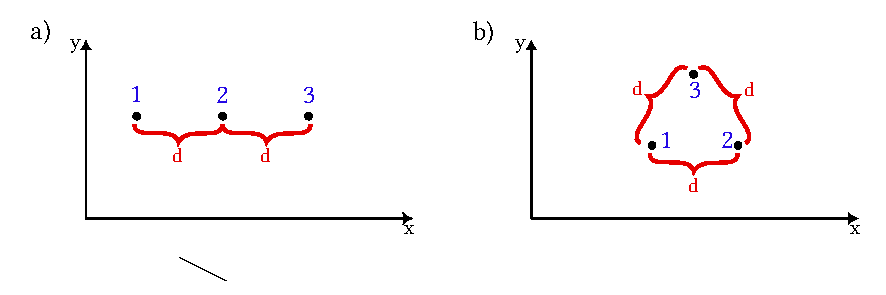
\includegraphics[width=0.9\textwidth]{./theory/physics/numerical-solutions/simple_case.pdf}}
    \vspace{-1cm}
    \caption{A representation of two simple latices. The spins are fixed at the point of the numbered locations. All sites have the same distance $d$ from their neighbors. Note, that a spin up \up is directed parallel to the z-axis. That means in this case it would point out of the paper in the direction of the viewer.}
    \label{fig:simpleThreeLatticeIsing}
\end{figure}

In the beginning one trivial example will be discussed. The lattice is visualized in \autoref{fig:simpleThreeLatticeIsing}a.
This corresponds to a linear lattice in 1D. Let the hamiltonian be the one in \autoref{eq:hamiltonianExampleA}.

\begin{equation}
    \label{eq:hamiltonianExampleA}
    \hamiltonian = \sigma^z_1\sigma^z_2 + \sigma^z_2\sigma^z_3
\end{equation}

This hamiltonian is anti-ferromagnetic ($J = +1$), therefore the energy $E$ in \autoref{eq:schroedinger-general} becomes minimal (largest magnitude with negative sign) when the spins always point into the opposite direction as their neighbors: $\ket{\up, \down, \up}$ or $\ket{\down, \up, \down}$. This is quite a crucial step, so validating this yourself is advised for someone without prior quantum mechanical experience.
The ground state therefore will be a \emph{superposition} consisting of equal parts $\ket{\up, \down, \up}$ and $\ket{\down, \up, \down}$ (\autoref{eq:solutionSimpleExample}). The factor $\frac{1}{\sqrt[]{2}}$ instead of the seemingly more obvious $\frac{1}{2}$ makes the wavefunction be \emph{normalized}. If it wasn't for the square root, \autoref{eq:base-orthonormal} would not be satisfied. This way it is satisfied, which can be tested.

\begin{equation}
    \label{eq:solutionSimpleExample}
    \ket{\Psi_\mathrm{gnd}} = \frac{1}{\sqrt[]{2}} \cdot \ket{\up, \down, \up} +  \frac{1}{\sqrt[]{2}} \cdot \ket{\down, \up, \down}
\end{equation}

The second example, visualized in \autoref{fig:simpleThreeLatticeIsing}b, however is not as simple. The corresponding hamiltonian can be seen in \autoref{eq:hamiltonianExampleB}.
\begin{equation}
    \label{eq:hamiltonianExampleB}
    \hamiltonian = \sigma^z_1\sigma^z_2 +\sigma^z_2\sigma^z_3 +\sigma^z_1\sigma^z_3
\end{equation}
It has one more interaction than the previous one. Even though it also is anti-symmetric, it is \emph{not} possible to align all three spins in a way, so that they stand anti-parallel to all their neighbors. This phenomenon is called \emph{frustration} \cite{frustration}.

Already this minimal problem has a complex superposition of eight base states as a ground state. The introduction of the transverse field will only make this more complex. Therefore a systematic way of finding the solution will be presented.

For this purpose, the example from \autoref{fig:simpleThreeLatticeIsing}b will be used once more, but this time with the hamiltonian in \autoref{eq:hamiltonianExampleTransverse}.
\begin{equation}
    \label{eq:hamiltonianExampleTransverse}
    \hamiltonian = J\cdot \sigma^z_1\sigma^z_2 +J\cdot\sigma^z_2\sigma^z_3 +J\cdot\sigma^z_1\sigma^z_3
    +h \sigma^x_1+h \sigma^x_2+h \sigma^x_3
\end{equation}

The goal is now, to write the hamiltonian \hamiltonian as a matrix. 
The elements of the matrix should be $\bra{m}\hamiltonian\ket{n}$. Where $\ket{m}$ and $\ket{n}$ are two states out of the chosen basis. In this case the eight base states are the following (\emph{canonical spin basis}):

\begin{center}
    \begin{tabular}{llll} 
        1: $\ket{\up, \up, \up}$ & 2: $\ket{\up, \up, \down}$  & 3: $\ket{\up, \down, \up}$  & 4: $\ket{\up, \down, \down}$ \\
        5: $\ket{\down, \up, \up}$ & 6: $\ket{\down, \up, \down}$  & 7: $\ket{\down, \down, \up}$  & 8: $\ket{\down, \down, \down}$ 
    \end{tabular}
\end{center}

In \autoref{eq:matrixElement} an example calculation of $\bra{2}\hamiltonian\ket{4}$ is presented.

\begin{equation}
    \label{eq:matrixElement}
    \begin{split}
        &\bra{\up, \up, \down} \hamiltonian \ket{\up, \down, \down} = \\\\ % new line
         \bra{\up, \up, \down} J\cdot \sigma^z_1\sigma^z_2 \ket{\up, \down, \down} +
         &\bra{\up, \up, \down} J\cdot \sigma^z_2\sigma^z_3 \ket{\up, \down, \down} +
         \bra{\up, \up, \down} J\cdot \sigma^z_1\sigma^z_3 \ket{\up, \down, \down} +\\
         \bra{\up, \up, \down} h\cdot \sigma^x_1 \ket{\up, \down, \down} +
         &\bra{\up, \up, \down} h\cdot \sigma^x_2 \ket{\up, \down, \down} +
         \bra{\up, \up, \down} h\cdot \sigma^x_3 \ket{\up, \down, \down}\stackrel{\ref{eq:pauli-transformation}, \ref{eq:pauli-many-body}}{=}\\\\ % new line
          \bra{\up, \up, \down} J\cdot  1 \cdot (-1) \ket{\up, \down, \down} +
         & \bra{\up, \up, \down} J\cdot (-1) \cdot (-1) \ket{\up, \down, \down} +
          \bra{\up, \up, \down} J\cdot  1 \cdot (-1) \ket{\up, \down, \down} +\\
          \bra{\up, \up, \down} h\cdot  1 \cdot \ket{\down, \down, \down} +
         & \bra{\up, \up, \down} h\cdot 1 \cdot \ket{\up, \up, \down} +
          \bra{\up, \up, \down} h\cdot  1 \cdot \ket{\up, \down, \up} =\\\\ % new line
          (-J)\cdot      \bra{\up, \up, \down}  \ket{\up, \down, \down} +
         & J\cdot        \bra{\up, \up, \down} \ket{\up, \down, \down} +
          (-J)\cdot      \bra{\up, \up, \down}  \ket{\up, \down, \down} +\\
          h\cdot         \bra{\up, \up, \down}  \ket{\down, \down, \down} +
         & h\cdot        \bra{\up, \up, \down} \ket{\up, \up, \down} +
          h\cdot         \bra{\up, \up, \down}  \ket{\up, \down, \up}\stackrel{\ref{eq:base-orthonormal}}{=}\\\\ % new line
          (-J)\cdot 0 + J\cdot 0 &+  (-J)\cdot 0 + h\cdot 0  + h\cdot 1 + h\cdot 0   = h 
    \end{split}
\end{equation}

Placing them inside a matrix at the corresponding location yields the matrix representation for $\bra{m}\hamiltonian\ket{n}$ that can be seen in \autoref{eq:matrix-hamiltonian}.
Because of \autoref{eq:base-factors}, each wavefunction can be written in terms of the chosen base. This is used in \autoref{eq:matrix-hamiltonian-vector}. By representing the wavefunction as a column vector, filled with the scaling factors, the transformation is complete. 
The calculation of the hamiltonian \hamiltonian acting on a wavefunction $\Psi$ as in \autoref{eq:schroedinger-general} can now be computed analogously by performing the matrix multiplication $\bra{m}\hamiltonian\ket{n} \cdot \Psi_\mathrm{vec}$.

\begin{equation}
    \label{eq:matrix-hamiltonian}
    \begin{pNiceMatrix}[first-row,first-col]
        &
        \ket{\up, \up, \up}&
        \ket{\up, \up, \down}&
        \ket{\up, \down, \up}&
        \ket{\up, \down, \down}&
        \ket{\down, \up, \up}&
        \ket{\down, \up, \down}&
        \ket{\down, \down, \up}&
        \ket{\down, \down, \down}\\
        \bra{\up, \up, \up}        \phantom{.} & 3 \cdot J  & h         & h         & 0         & h         & 0         & 0         & 0   \\
        \bra{\up, \up, \down}      \phantom{.} & h          &-1 \cdot J & 0         & h         & 0         & h         & 0         & 0   \\
        \bra{\up, \down, \up}      \phantom{.} & h          & 0         &-1 \cdot J & h         & 0         & 0         & h         & 0   \\
        \bra{\up, \down, \down}    \phantom{.} & 0          & h         & h         &-1 \cdot J & 0         & 0         & 0         & h   \\
        \bra{\down, \up, \up}      \phantom{.} & h          & 0         & 0         & 0         &-1 \cdot J & h         & h         & 0   \\
        \bra{\down, \up, \down}    \phantom{.} & 0          & h         & 0         & 0         & h         &-1 \cdot J & 0         & h   \\
        \bra{\down, \down, \up}    \phantom{.} & 0          & 0         & h         & 0         & h         & 0         &-1 \cdot J & h   \\
        \bra{\down, \down, \down}  \phantom{.} & 0          & 0         & 0         & h         & 0         & h         & h         & 3 \cdot J \\
    \end{pNiceMatrix}
\end{equation}

\begin{equation*}
    \begin{split}
        \Psi = 
            &c_1 \ket{\up, \up, \up}  +
            c_2 \ket{\up, \up, \down}  +
            c_3 \ket{\up, \down, \up}  +
            c_4 \ket{\up, \down, \down}  +\\
            &c_5 \ket{\down, \up, \up} +
            c_6 \ket{\down, \up, \down}  +
            c_7 \ket{\down, \down, \up}  +
            c_8 \ket{\down, \down, \down}
    \end{split}
\end{equation*}
\begin{equation} % this is very bad style, but it would not for the life me let this stuff be aligned properly
    \label{eq:matrix-hamiltonian-vector}        
    \longrightarrow\\
\end{equation}
\begin{equation*}
    \begin{split}
        \Psi_\mathrm{vec} = 
        \begin{pNiceMatrix}[first-row]
            \ket{\up, \up, \up}&
            \ket{\up, \up, \down}&
            \ket{\up, \down, \up}&
            \ket{\up, \down, \down}&
            \ket{\down, \up, \up}&
            \ket{\down, \up, \down}&
            \ket{\down, \down, \up}&
            \ket{\down, \down, \down}\\
            c_1&   
            c_2&
            c_3&
            c_4&
            c_5&
            c_6&
            c_7&
            c_8
        \end{pNiceMatrix} \raisebox{0.7em}{T}
    \end{split}
\end{equation*}

Rewriting \autoref{eq:schroedinger-general} in terms of the newly defined matrix operators, results in \autoref{eq:schroedinger-matrix}.
\begin{equation}
    \label{eq:schroedinger-matrix}
    \bra{m}\hamiltonian\ket{n} \cdot \Psi_\mathrm{vec} = E \cdot \Psi_\mathrm{vec}
\end{equation}

This representation is quite useful, because now the problem of finding the eigenstates has been turned into a problem of finding the eigenvectors for a sparse (hermitian) matrix. 
A problem, that is already solved by a lot of algorithms and software \cite{scipyeigsh}.
It is now clear, that the smallest eigenvalue of the matrix \emph{is} the ground state energy and the corresponding eigenvector \emph{is} a representation for the ground state wavefunction.

As mentioned, the complexity of the problem does not lie in terms of how to compute this value, but in how to compute it in reasonable time.
If $L$ is the size of the lattice, it is obvious, that the canonical base contains $2^L$ states ($L$ sites, each can be \up or \down).
Therefore the matrix whose eigenvalues are required has $2^{2\cdot L}$ entries, of which $2^L \cdot m$ are non-zero ($m$ being constant and dependent on the form of the hamiltonian, as well as the number of neighbors to one site in the lattice). 

So even \emph{if} a algorithm was found, to compute the eigenvalues of such a matrix in linear time (in comparison to the number of non-zero entries in the matrix), the time complexity for solving the problem would still scale in $\mathcal{O} (2^L)$ with the number of lattice sites $L$.

To compute macroscopic crystals, the number of lattice sites would have to be in the same range of magnitude as \emph{Avogadros constant} ($N_\mathrm{A} \approx \SI{6.022E23}{\per\mol}$ \cite{avogadrosNumber}). Current hardware can not go reasonably into the range of hundreds. 

This naive algorithm is implemented in \filepath{\cite{selfPhysics}}{/computation/numerical\_solution.py}. On moderately modern hardware it takes about \SI{2.5}{\minute} to compute the ground state energy of a $L=13$ lattice. $L=16$ already takes hours.
        \FloatBarrier
        \subsection{Solutions with Neural Quantum States}
        \label{sec:theory-neuralquantumstates}
        As a direct numerical approach is not sufficient, more advanced methods needed to be developed. 
\emph{Iterative} approaches have shown to be quite effective. 
In these kind of methods, the goal is not to compute a full solution directly, but to start with a random solution and perform iterative updates to it. 
If a good update strategy is chosen, the solution may converge towards the desired solution.

Because of the iterative nature, it is not necessary to do a complete computation at once. 
As learned in \fullref{sec:theory-numericalsolution}, the memory requirement for storing a complete hamiltonian matrix representation is also exponential.
So even with unlimited time, a numerical calculation could be impossible because of limited available memory. 
The iterative methods get around this, by being able to chose a data structure with much higher information density than the full hamiltonian (For example if only the ground state is wanted, it is unnecessary to store anything but information regarding it. The hamiltonian though encodes a lot of \glqq unnecessary\grqq{} information about other states). This structure can then be iteratively refined.

In practice a so called \emph{neural quantum state} (NQS) is used. 
This basically is nothing but a neural network, taken from established machine learning tasks \cite{restrictedBoltzmanMachines}.
The function is parametrized by $M$ variables $\theta_i \in \mathbb{R}, 0\leq i < M$ and takes a spin configuration as an input.
A spin configuration for $N$ lattice sites can be described by $\sigma_j \in \left\{\up, \down\right\}, 0\leq j < N$.
The function will be written like \autoref{eq:parametrized-wavefunction}.

\begin{equation}
    \label{eq:parametrized-wavefunction}
    \ket{\Psi_{\theta_0, ..., \theta_{M-1}}(\sigma_0, ..., \sigma_{N-1})} \equiv \ket{\Psi_\theta}
\end{equation}

In order to compute a helpful representation, the identities \autoref{eq:completeness-of-base} and \autoref{eq:wave-function-probability} are necessary \cite{schwablQM}. \autoref{eq:completeness-of-base} applies to \emph{complete orthonormal} bases only.

\begin{equation}
    \label{eq:completeness-of-base}
    \sum\limits_{s} \ket{s}\bra{s} = \mathbb{1}
\end{equation}

\begin{equation}
    \label{eq:wave-function-probability}
    \bra{\Psi}\ket{\Psi} = \Psi^\ast\cdot \Psi = \left|\Psi\right|^2 \in \mathbb{R}
\end{equation}

The following method is described in \cite{jVMCPaper}.

To calculate the \emph{expectation value} of a quantum mechanical operator \operator for the wavefunction $\ket{\Psi}$, the expression 
$\frac{\bra{\Psi}\operator\ket{\Psi}}{\bra{\Psi}\ket{\Psi}}$ is used \cite{schwablQM}. The denominator assures, that the calculation is correct for \emph{non-normalized} wavefunctions (as the NQS is initialized randomly it very likely isn't normalized). 

Applying this to the problem at hand, the target is to measure the observable corresponding to \operator in the parametrized neural quantum state $\ket{\Psi_\theta}$.

\begin{equation}
    \label{eq:derivation-local-estimator}
    \begin{split}
        \frac{\bra{\Psi_\theta}\operator\ket{\Psi_\theta}}{\bra{\Psi_\theta}\ket{\Psi_\theta}} &\stackrel{\ref{eq:completeness-of-base}}{=}
        %
        \frac{\bra{\Psi_\theta} \left(\sum\limits_{s} \ket{s}\bra{s}\right)
        \operator \left(\sum\limits_{s'} \ket{s'}\bra{s'}\right) \ket{\Psi_\theta}}{\bra{\Psi_\theta}\left(\sum\limits_{s} \ket{s}\bra{s}\right)\ket{\Psi_\theta}}\\
        %
        &\stackrel{\phantom{\ref{eq:completeness-of-base}}}{=}
        \frac{\sum\limits_{s, s'} \bra{\Psi_\theta} \ket{s}\bra{s}
        \operator \ket{s'}\bra{s'} \ket{\Psi_\theta}}{\sum\limits_{s}\bra{\Psi_\theta}\ket{s}\bra{s}\ket{\Psi_\theta}}
        %
        \stackrel{\phantom{\ref{eq:completeness-of-base}}}{=}
        \frac{\sum\limits_{s} \bra{\Psi_\theta} \ket{s} \frac{\bra{s} \ket{\Psi_\theta}}{\bra{s} \ket{\Psi_\theta}} \sum\limits_{s'} \bra{s}
        \operator \ket{s'}\bra{s'} \ket{\Psi_\theta}}{\sum\limits_{s}\bra{\Psi_\theta}\ket{s}\bra{s}\ket{\Psi_\theta}}\\
        %
        &\stackrel{\phantom{\ref{eq:completeness-of-base}}}{=}
        \sum\limits_{s} \frac{ \bra{\Psi_\theta} \ket{s}\bra{s} \ket{\Psi_\theta} \sum\limits_{s'} \bra{s}
        \operator \ket{s'} \frac{\bra{s'} \ket{\Psi_\theta}}{\bra{s} \ket{\Psi_\theta}}}{\bra{\Psi_\theta}\ket{s}\bra{s}\ket{\Psi_\theta}}
        %
        \stackrel{\ref{eq:local-estimator}}{=}
        \sum\limits_{s} \frac{ \bra{\Psi_\theta} \ket{s}\bra{s} \ket{\Psi_\theta} \operator_\mathrm{loc}^\theta(s)}{\bra{\Psi_\theta}\ket{s}\bra{s}\ket{\Psi_\theta}}\\
        %
        &\stackrel{\ref{eq:base-factors}}{=}
        \sum\limits_{s} \frac{ \Psi_\theta(s)^\ast \cdot \Psi_\theta(s) \cdot \operator_\mathrm{loc}^\theta(s)}{\Psi_\theta(s)^\ast \cdot \Psi_\theta(s)}
        %
        \stackrel{\ref{eq:wave-function-probability}}{=}
        \sum\limits_{s} \frac{ \left|\Psi_\theta(s)\right|^2  \operator_\mathrm{loc}^\theta(s)}{\left|\Psi_\theta(s)\right|^2}
    \end{split}
\end{equation}

In the derivation, the \emph{local estimator} (\autoref{eq:local-estimator}) is introduced. Because the computational base is sparse, only very few elements of the sum over $s'$ in \autoref{eq:local-estimator} are non-zero \cite{jVMCPaper}. A local estimator can therefore be evaluated in constant time.

\begin{equation}
    \label{eq:local-estimator}
    \operator_\mathrm{loc}^\theta(s) = \sum\limits_{s'} \bra{s} \operator \ket{s'} \frac{\bra{s'} \ket{\Psi_\theta}}{\bra{s} \ket{\Psi_\theta}}
\end{equation}

The final result in \autoref{eq:derivation-local-estimator} has the form of a \emph{probability distribution} over $s$.
So the calculation of a expectation value can be re-formulated as the calculation of the expectation value of $s$ of the local estimator (which can be evaluated in constant time).

This alone is not helpful, because $\ket{s}$ is still exponentially large in regards to the problem size.
But this shortcoming can be resolved with the introduction of \emph{Monte Carlo} sampling.
The \emph{probability density} can be estimated, by looking at only a subset of possible $\ket{s}$.

By randomly sampling a large, but manageable number $N_\mathrm{MC}$ of states $s_{(n)}$ with the \emph{Metropolis algorithm} \cite{quantumMonteCarloSimulationsOfSolids}, the true value can be approximated (\autoref{eq:mc-local-estimator}) \cite{jVMCPaper}.

\begin{equation}
    \label{eq:mc-local-estimator}
    \frac{\bra{\Psi_\theta}\operator\ket{\Psi_\theta}}{\bra{\Psi_\theta}\ket{\Psi_\theta}} \approx
    \frac{1}{N_\mathrm{MC}} \sum\limits_{n=1}^{N_\mathrm{MC}} \operator_\mathrm{loc}^\theta(s_{(n)})
\end{equation}

Therefore the energy of a system can be estimated with \autoref{eq:energy-optimization}. All the terms can efficiently be computed, using methods from \fullref{sec:theory-numericalsolution}.

\begin{equation}
    \label{eq:energy-optimization}
    E(\theta) = \frac{\bra{\Psi_\theta}\hamiltonian\ket{\Psi_\theta}}{\bra{\Psi_\theta}\ket{\Psi_\theta}} \approx
    \frac{1}{N_\mathrm{MC}} \sum\limits_{n=1}^{N_\mathrm{MC}} \hamiltonian_\mathrm{loc}^\theta(s_{(n)}) \stackrel{\ref{eq:local-estimator}}{=}
    \frac{1}{N_\mathrm{MC}} \sum\limits_{n=1}^{N_\mathrm{MC}} \left(\sum\limits_{s'} \bra{s_{(n)}} \hamiltonian \ket{s'} \frac{\bra{s'} \ket{\Psi_\theta}}{\bra{s_{(n)}} \ket{\Psi_\theta}}\right)
\end{equation}

As it is known, that the ground state energy $E_0$ is the smallest energy, the ground state can be estimated in the following way:
\begin{enumerate}
    \setlength\itemsep{-0.5em}
    \item Start with a randomly initialized NQS
    \item Estimate its energy with \autoref{eq:energy-optimization} and MC-sampled states
    \item Calculate the neural network error, assuming $E(\theta)$ should be smaller (formula in \cite{jVMCPaper})
    \item Propagate the error back into the network
    \item Repeat at 2. with the updated NQS
\end{enumerate}

Because the method iteratively updates the network by performing tiny variations, it is called \emph{variational Monte Carlo} (VMC) method.

        \FloatBarrier
        \subsection{Imaginary Time Evolution}
        \label{sec:theory-imaginarytimeevolution}
        Many different iterative methods are being employed to calculate the desired physical quantities.
In this section, a mathematical idea will be discussed, that has several applications.
The method is employed in the \emph{diffusion Monte Carlo} method (DMC) \cite{quantumMonteCarloSimulationsOfSolids}, a second application of Monte Carlo sampling in comparison to VMC.

This section is about more advanced quantum mechanical principles and requires prior experiences. It is of supplemental nature and can therefore be skipped without sacrificing on the possibility to understand subsequent parts of the thesis.

The method is described in \cite{imaginarySchroedingerEquation}.

\autoref{eq:schroedinger-general} can be generalized to be no longer time independent. 
\autoref{eq:schroedinger-td} is called the \emph{time-dependent Schrödinger equation}. $\hbar$ is the \emph{reduced Planck constant}, $t$ is the time.

\begin{equation}
    \label{eq:schroedinger-td}
    \hamiltonian \ket{\Psi(t)} = i\hbar \frac{\partial }{\partial t} \ket{\Psi(t)}
\end{equation}

In this case, the wavefunction also needs to depend on the time as a variable.
For a time-independent hamiltonian, the time dependent wavefunction can be obtained via \autoref{eq:timeEvolutionWavefunction} \cite{schwablQM} with the energy eigenvalues $E_n$ ($E_0$ being the ground state energy), the energy eigenbase states $\ket{n}$ and the wavefunction at time $t=0$, $\ket{\Psi(0)}$.

\begin{equation}
    \label{eq:timeEvolutionWavefunction}
        \ket{\Psi(t)} = e^{-i\hamiltonian t / \hbar} \ket{\Psi(0)}
\end{equation}

That \autoref{eq:timeEvolutionWavefunction} is a solution to \autoref{eq:schroedinger-td} can be verified like in \autoref{eq:validationTimeEvolution} (notice that the hamiltonian is time-independent).

\begin{equation}
    \label{eq:validationTimeEvolution}
    \begin{split}
        i\hbar \frac{\partial }{\partial t} \ket{\Psi(t)} &\stackrel{\ref{eq:timeEvolutionWavefunction}}{=} 
        i\hbar \frac{\partial }{\partial t}  e^{-i\hamiltonian t / \hbar} \ket{\Psi(0)}\\
        &\stackrel{\phantom{\ref{eq:timeEvolutionWavefunction}}}{=} \frac{-i\cdot i \hamiltonian \hbar}{\hbar} e^{-i\hamiltonian t / \hbar} \ket{\Psi(0)}\\
        &\stackrel{\ref{eq:timeEvolutionWavefunction}}{=} \hamiltonian \ket{\Psi(t)}
    \end{split}
\end{equation}

\autoref{eq:timeEvolutionWavefunction} can be rewritten in terms of the energy eigenbase.

\begin{equation}
    \label{eq:rewriteTimeEvolutionWavefuntion}
    \begin{split}
        \ket{\Psi(t)} &\stackrel{\phantom{\ref{eq:base-change}, \ref{eq:base-factors}}}{=} e^{-i\hamiltonian t / \hbar} \ket{\Psi(0)} \\
        &\stackrel{\ref{eq:base-change}, \ref{eq:base-factors}}{=}
        \sum\limits_{n}^{} e^{-i \hamiltonian t / \hbar} \bra{n}\ket{\Psi(0)} \ket{n}\\
        &\stackrel{\phantom{\ref{eq:base-change}, \ref{eq:base-factors}}}{=}
        \sum\limits_{n}^{} e^{-i E_n t / \hbar} \bra{n}\ket{\Psi(0)} \ket{n}
    \end{split}
\end{equation}

In \autoref{eq:rewriteTimeEvolutionWavefuntion}, an operator gets applied from inside an exponent. This can be explained with the possibility to express the $e$-function in terms of its \emph{Taylor series} \cite{schwablQM}. This is important to understand the transition from \hamiltonian to $E_n$ in the exponent. For the transformation, the function is written as its Taylor series, the operator gets applied and then the Taylor series is reversed into the function. Remember that $\bra{n}\ket{\Psi(0)}$ is simply a complex number.

The method is called \emph{imaginary} time evolution, because of the step in \autoref{eq:complexTimeVariableChange}.

\begin{equation}
    \label{eq:complexTimeVariableChange}
    \tau = i\cdot t
\end{equation}

An \glqq imaginary\grqq{} time $\tau$ can be obtained by equation \autoref{eq:complexTimeVariableChange}. Switching variables in \autoref{eq:rewriteTimeEvolutionWavefuntion} leads to the representation shown in \autoref{eq:complexTimeExponential}.

\begin{equation}
    \label{eq:complexTimeExponential}
    \ket{\Psi(\tau)} = \sum\limits_{n}^{} e^{-E_n \tau / \hbar} \bra{n}\ket{\Psi(0)} \ket{n}
\end{equation}

$E_0 > 0$ can be assumed without loss of generality.
It is known by definition, that $E_0 \leq E_j, j\neq 0$. 
\autoref{eq:complexTimeExponential} contains only terms, that decay exponentially with $\tau$.
Because of that, for large values of $\tau$ all terms decay to 0, but the $n=0$ term decays the slowest. \autoref{eq:complexTimeApplication} is therefore won.

\begin{equation}
    \label{eq:complexTimeApplication}
    \lim\limits_{\tau \rightarrow \infty}\frac{\ket{\Psi(\tau)}}{e^{-E_0 \tau / \hbar}} \stackrel{\ref{eq:complexTimeExponential}}{=} \bra{0}\ket{\Psi(0)} \ket{0}
\end{equation}

This means, that if the starting wavefunction has an overlap with the ground state ($\bra{0}\ket{\Psi(0)} \neq 0$), if the wavefunction is evolved in imaginary time, all contributions except the ground state contribution will be eliminated.

This can be used to find the ground state \cite{quantumMonteCarloSimulationsOfSolids}. A random starting function is chosen and evolved in complex time with the aid of Monte Carlo sampling. The ground state can then be extracted. If there is no overlap between the starting function and the ground state, the method converges to the base state with the smallest energy that also has overlap.
        \FloatBarrier
        \subsection{Explored Lattice Patterns}
        \label{sec:theory-latticepatterns}
        In \autoref{fig:simpleThreeLatticeIsing} two examples of lattice-shapes were already introduced.
In the research leading to this thesis, a selection of lattices was chosen.
The implementation supports a 1D lattice (the default \textbf{linear} lattice/chain  (\autoref{fig:appendix-linear-lattices})) and five different 2D lattices 
(\textbf{cubic} (\autoref{fig:appendix-cubic-lattices}), \textbf{hexagonal} (\autoref{fig:appendix-hexagonal-lattices}), \textbf{trigonal\_square} (\autoref{fig:appendix-trigonal_square-lattices}), \textbf{trigonal\_hexagonal} (\autoref{fig:appendix-trigonal_hexagonal-lattices}) and \textbf{trigonal\_diamond} (\autoref{fig:appendix-trigonal_diamond-lattices})).

The lattice structure can be interactively visualized with the use of \cite{selfPhysics} \filepath{/structures/visualize.py}.
The same code was used to generate the referenced visualization printed in the \nameref{sec:appendix}.
The construction of the hexagonal lattice types, makes use of the hexagonal coordinate systems defined in \cite[]{hexagonalGrids}.

The numbers, that can be seen in the visualization denote the location-index of the memory, that is responsible for carrying the spin state at that lattice site in the later representation. As will become obvious in \fullref{sec:theory-graphs}, the structure of a lattice cannot always be represented directly analogous in memory. Therefore an alternative way of addressing lattice sites and their surroundings needs to be employed.
In this case, the framework generates the set of \emph{nearest neighbor} (marked green in the visualization) and \emph{next-nearest neighbor} (marked yellow in the visualization) indices for a given lattice site (marked red in the visualization). These are used as structural inputs for later discussed \emph{graph} architectures.

A quite important feature for the physical aspect of the calculation is the \emph{periodicity} of a lattice. 
As real world crystals have many magnitudes more lattice sites than can be currently simulated, \emph{boundary effects} play a significant role in simulated lattices.
This often times is an unwanted manner, if the goal is to calculate the behavior of the system far away from the edges. 
In that region, lattices should have the property of \emph{translational symmetry}. 
To aid with this, a \emph{periodic} repetition of the lattice can be toggled. 
It is responsible for defining neighbors for lattice sites close to the edges of the lattice.
The \nameref{appendix:lattice-visualisation} in the appendix shows this, by providing the information whether the pictured lattice is periodic or not.

The way in that the lattices are tiled should become clear from the visualization.
It is noteworthy, that the \textbf{cubic}, \textbf{trigonal\_square} and \textbf{trigonal\_diamond} lattices have repetition along two axes, while the \textbf{hexagonal} and \textbf{trigonal\_hexagonal} have three. 
The hope is that the \textbf{trigonal\_hexagonal} and \textbf{trigonal\_square}/\textbf{trigonal\_diamond} lattices show the same behavior in non-periodic mode (as they all three represent a trigonal lattice), while differences manifest in periodic inspection.

Last, there is a setting to \emph{randomly swap} lattice positions. 
The effect of this can be seen in \autoref{fig:direct-comparison-lattice-site-swaps}.

\begin{figure}[htbp]
    \centering
    \makebox[\textwidth][c]{
        \includegraphics[width=0.3\textwidth]{./theory/physics/explored-lattice-patterns/hexagonal,size=2,np.pdf}
        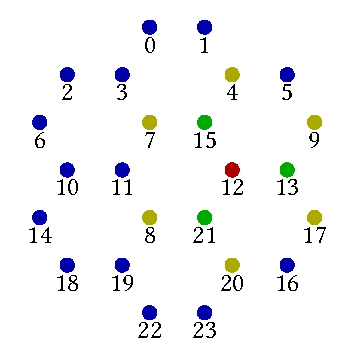
\includegraphics[width=0.3\textwidth]{./theory/physics/explored-lattice-patterns/hexagonal,size=2,np,rs=2.pdf}
    }
    \makebox[\textwidth][c]{
        \includegraphics[width=0.3\textwidth]{./theory/physics/explored-lattice-patterns/trigonal_square,size=3,np.pdf}
        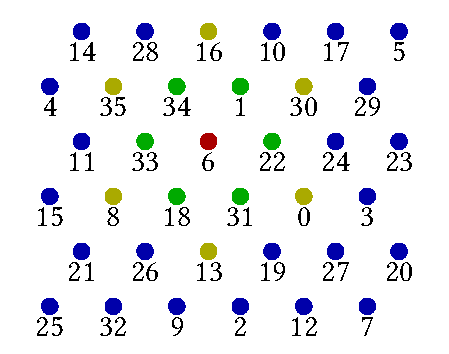
\includegraphics[width=0.3\textwidth]{./theory/physics/explored-lattice-patterns/trigonal_square,size=3,np,rs=-1.pdf}
    }

    \vspace{0.2cm}
    \caption{Visualization of the property \emph{random swaps} of the lattice structure helper. In the first set of figures, two swaps were performed on a hexagonal lattice of size 2 (8 with 15 and 16 with 21). The neighbor-index calculation takes this into effect, therefore the highlighted lattice sites do not change. The second set of figures shows the setting -1 for a trigonal\_square lattice of size 3. This basically makes the generator perform such a high number of pair swaps, that the index-position correlation can be assumed to be random. 
    }
    \label{fig:direct-comparison-lattice-site-swaps}
\end{figure}

The goal of this setting is to decouple the in-memory representation and the structure of the simulated lattice. 
Effects of this will be explored in \fullref{sec:experiments-resiliencylatticeencoding}.

General data about the lattices is provided in \autoref{table:lattice-information}.

\begin{table}[htbp]
    \centering
    \begin{tabular}{l|cc|ccccccc} 
        \toprule
        Lattice name & \#nn & \#nnn &$L$(1)&$L$(2)&$L$(3)&$L$(4)&$L$(5)&$L$(6)&$L$(7)\\  
        \midrule 
        linear & 2 & 2 & 1 & 2 & 3 & 4 & 5 & 6 & 7\\
        cubic & 4 & 4 & 4 & 9 & 16 & 25 & 36 & 49 & 64\\
        trigonal\_square & 6 & 6 & 4 & 16 & 36 & 64 & 100 & 144 & 196\\
        trigonal\_diamond & 6 & 6 & 4 & 9 & 16 & 25 & 36 & 49 & 64\\
        trigonal\_hexagonal & 6 & 6 & 7 & 19 & 37 & 61 & 91 & 127 & 169\\
        hexagonal & 3 & 6 & 6 & 24 & 54 & 96 & 150 & 216 & 294\\
        \bottomrule
    \end{tabular}
    \vspace{0.5cm}
    \caption{General information about the explored lattices. \textbf{\#nn} describes the number of nearest neighbors, \textbf{\#nnn} the number of next nearest neighbors. The numbers describe the maximum possible neighbor count. If a lattice is non-periodic, some sites can have less neighbors. $L(i)$ describes the number of lattice sites for a lattice of \textbf{size=$i$}}.
    \label{table:lattice-information}
\end{table}





        \FloatBarrier
    \section{From the Perspective of Computer Science}
        \label{sec:theory-cs}
        The first set of experiments will be on the image classification task.
The goal will be to compare the architectural advantages and drawbacks between multiple different kinds of metaformers.

Training was be performed on a subset of 100 classes from the \emph{ImageNet} dataset \cite{imagenetDataset}.
The accompanying code to replicate these experiments can be found on GitHub \cite{selfComputerScience}.

The neural networks, as well as the training and evaluation code were written in python.
The \emph{PyTorch} \cite{pytorchGithub} machine learning framework was used as a measure to efficiently define neural networks and lever the computational capabilities of parallelization via GPUs.

The main metaformer model was originally based on the vision transformer found in an implementation of \emph{DINO} \cite{dinoGithub}, was however heavily modified. 
A comparison between the stock DINO model and the modified version will be also performed.
This however is not supposed to be a direct discrediting of any of the models, as their main purposes do not exactly align.
Therefore one or the other may excel in specific tasks.
Also a comparison against a pre-implemented \emph{poolformer} \cite{poolformerGithub} will be performed.

The \emph{einops} package \cite{einopsGithub} is heavily used. It provides tensor operations, configurable with the \emph{Einstein notation} and simplifies the notation and subsequently readability.
Lastly, the implementation of the \emph{positional encoding} is provided by \cite{positionalEncodingGithub}.

        \FloatBarrier
        \subsection{The Image Classification Task}
        \label{sec:theory-imageclassification}
        It has been more than 30 years, since it was proven, that already simple neural network architectures can in fact be \emph{universal approximators} \cite{ffnUnversalApproximator}. 
That means that if a problem can be formulated as a mathematical function, this function can be approximated by a neural network.
This has huge consequences, because if input and output are encoded digitally in a predefined format, \emph{all} mappings between these can be formulated in form of a mathematical function. 
Be it only the trivial one, that maps each input encoding to the desired output encoding.
Because of that, seemingly impossibly complex problems can be tackled nowadays. 

Part of the experimentation in the thesis will focus on the application of a select breed of neural networks on the \emph{image classification task}.
This is not a novel problem, but one that has been tried and solved by many teams of researchers. 
The gist is to build a neural network that can label the things pictured on some kind of image.
In our case an even simpler version of the problem will be considered. 
The only job of the network is to select one of $N$ predefined labels, that describes the picture best.

A generalization of the task pipeline can be viewed in \autoref{fig:image-classification-general}.

\begin{figure}[htbp]
    \centering
    \makebox[\textwidth][c]{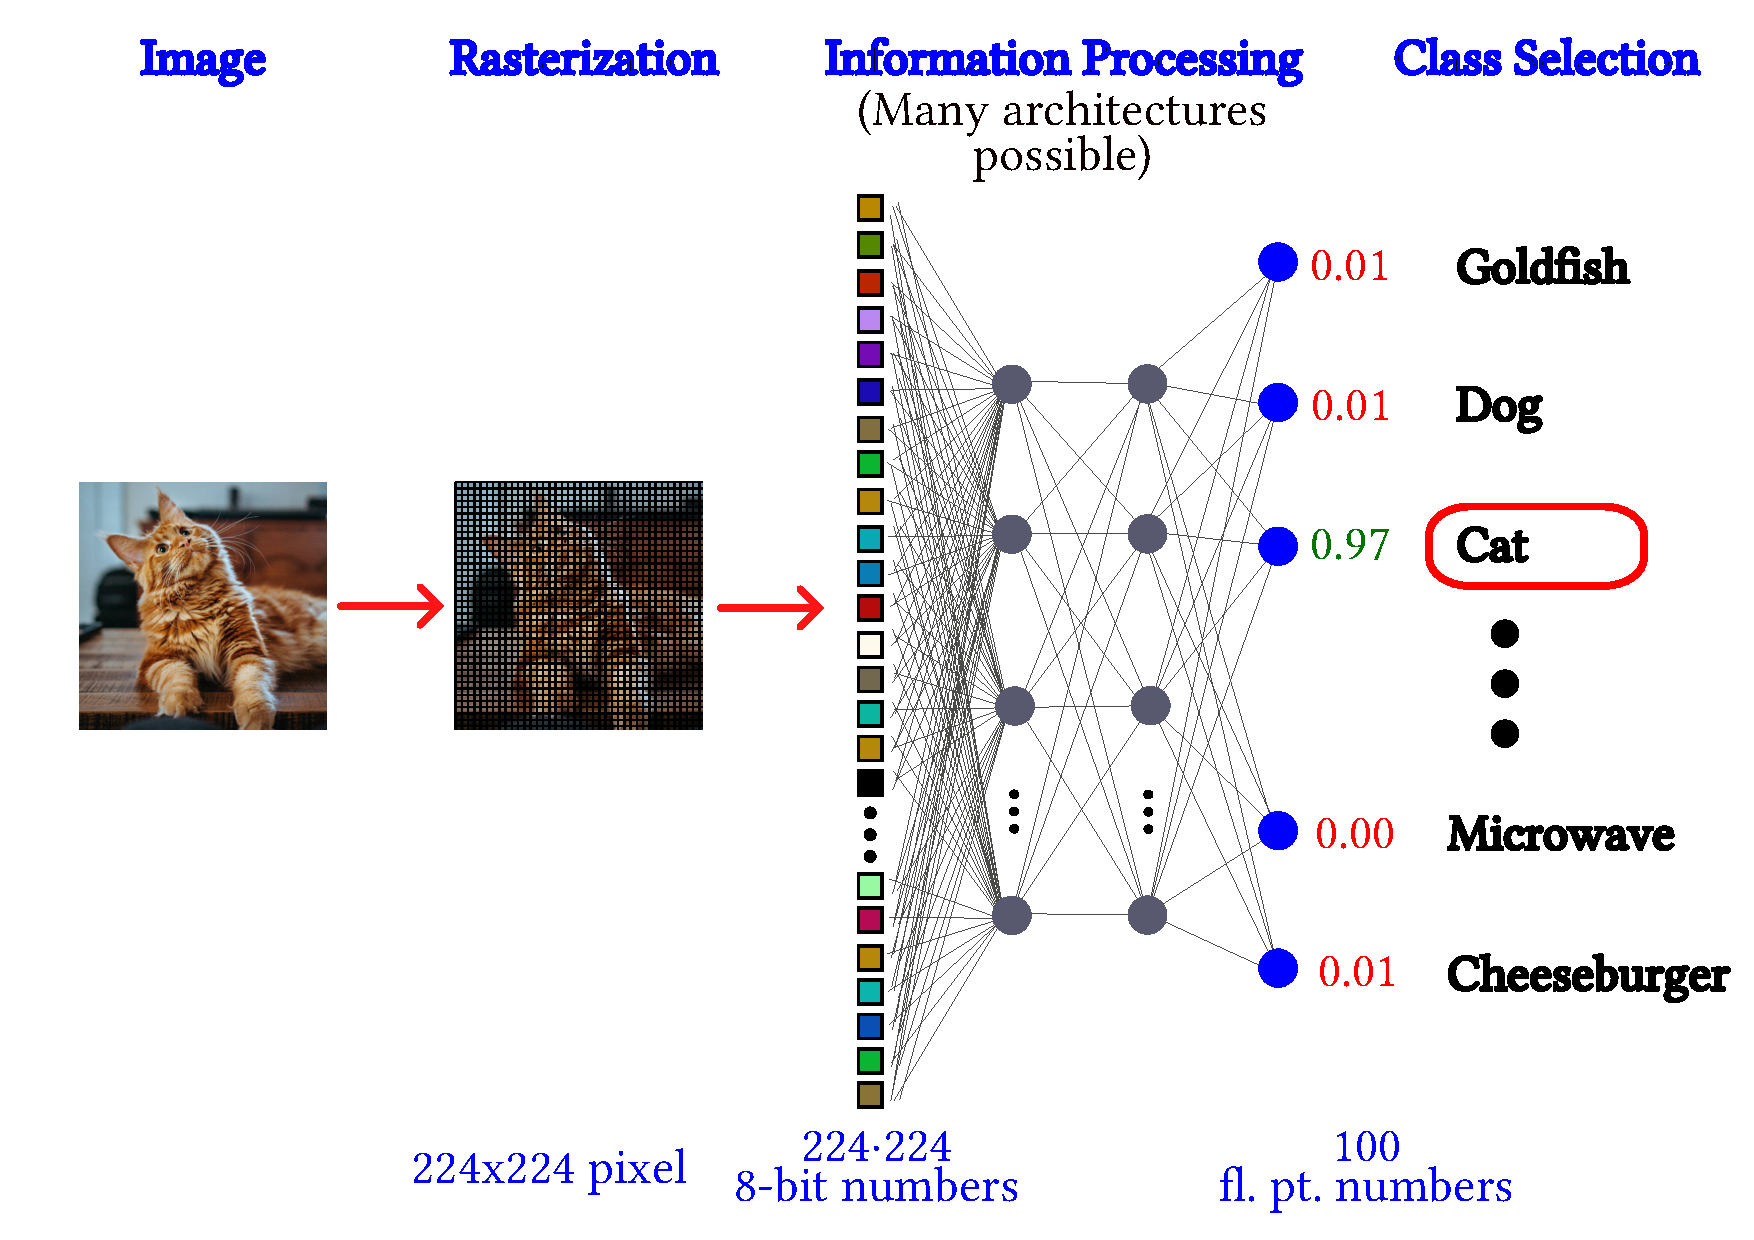
\includegraphics[width=\textwidth]{./theory/cs/image-classification/process.pdf}}
    \caption{Generalized schema of the image classification pipeline used in the experiments section of this thesis.
        The image gets rasterized, resized to 224$\times$224 pixel and 8 bit color depth per each of the three color channels. Then the image is normalized, reshaped into vector form and processed from there. The MLP in this image is only a placeholder. Many of the later discussed neural network architectures treat the reshaping, casting and processing differently. The output for all networks needs to be in form of 100 floating point numbers. The one closest to 1 gets selected as the networks choice. The class name the index represents can then be looked up.
        Cat image from \cite{catPhoto}.
    }
    \label{fig:image-classification-general}
\end{figure}

The aforementioned trivial mapping of inputs to outputs is obviously not feasable in reality, as for a $224\times 224$ pixel 8-bit grayscale image the function would need to consist of $256^{224\cdot 224} \approx \SI[]{7e120835}[]{}$ cases, most of which do not even make sense in terms of the predefined categories or even define a realistically possible image.

In order to solve the problem, the mapping function is \emph{approximated} with a neural network. 

To train the network, a pre-labeled set of training images is passed through it, the results are compared to the labels and the error is used to iteratively update the network with use of the \emph{backpropagation algorithm} \cite{machineLearningMitchell}, therefore improving the performance of the network in the next step.

A big challenge in training these kinds of networks is getting a sufficient amount of labeled training data. 
Today a lot of publicly available, high quality datasets exist for download. 
In this case, the \emph{CIFAR-10} \cite{cifarDataset} dataset was used for the first steps in the methods. 
A subset of \emph{100 classes} from the \emph{ImageNet} \cite{imagenetDataset} dataset was used in the experiments that were used to evaluate the general functionality of the explored network architectures.
The subset of chosen classes can be viewed in \filepath{\cite{selfComputerScience}}{/managing\_imagenet\_data/used\_synsets.txt}.

In the task the \emph{accuracy} describes the percentage of validation images whose label was guessed correctly by the network. It is not allowed to use the validation images during training. That way, the network only would need to memorize a tiny amount of images to perform good on the test. This is undesirable behavior, as the general idea is to teach the network to be able to classify previously unseen images in the right way. The \emph{training accuracy} is the analogous value, but calculated for the training images - that \emph{are} used during training (Because of that, this accuracy is often way higher).
The \emph{top-3-accuracy} is the percentage of validation images, for that the correct label was among the top three highest valued choices of the network. The same is true analogously for the \emph{top-5-accuracy}.
        \FloatBarrier
        \subsection{Neural Network Training}
        \label{sec:theory-neuralnetworktraining}
        When initializing neural networks, they most often come only with an empty structure, that allows for the possibility to acquire a computing machine if all the internal parameters and weights are set accordingly.
For very small computational networks, it is possible to set the weights by hand.
But already for low tens or hundreds of numbers this becomes an unfeasible task. 

Because of that, neural networks are \emph{trained} to get them into a working state. In the training phase the structure of the network is (normally) left static, only the parameter values are adjusted. 
The algorithm that accomplishes an update of the weights, that nudges the network \emph{towards} the desired solution, is called \emph{backpropagation} \cite{machineLearningMitchell}.
It is based on the chain rule of differentiation and uses the severity of changes a parameter inflicted on a (intermediate) result, to update the parameter in a way, that steers said result towards the desired one. 

As mentioned, for one run the structure is typically unchanged. 
The general shape of the network and many turning knobs on the update process can be controlled to allow for a more efficient representation and weight update.
The controlling variables are called \emph{hyperparameters}.
The most important hyperparameters in the later experiments will be the \emph{optimizer} (\emph{stochastic gradient descent} and \emph{adamw} \cite{adamwOptimizer} are compared), the \emph{loss function} (\emph{cross entropy loss} is used), and the \emph{batch size}. 
Additionally, the \emph{learning rate}, \emph{weight decay}, \emph{dampening} and \emph{momentum} can be set to modify the behavior of the optimizer.

Different optimizers change the updating behavior of the network. 
The loss function defines a measure on how far or close the computed solution is to the known solution.
The learning rate defines the step size that gets taken towards the target in one iteration.
Choosing its value too small results in slow convergence, choosing a value too big can result in overshooting and subsequently also lowering the speed of convergence.
Dampening and momentum are generally used to combat either of these effects.
Weight decay generally helps against \emph{overfitting} (If a model's generalization capacity is exhausted or the training examples are to monotone, this can lead to memorization of a subset of training examples. This increases the performance on training data, but hurts the performance on unseen data). 
As for our applications, overfitting is unimportant or even desired (see \autoref{sec:biases}), this parameter left unchanged.

The article \emph{A ConvNet for the 2020s} \cite{convNetForThe2020s} makes the point, that by heavily investing in choosing the appropriate hyperparameters, state of the art performance can be extracted even from \glqq standard\grqq{} model architectures. 
As the focus in this thesis is to compare the performance of different \emph{architectures} with each other, \emph{no efforts} are made to tune hyperparameters to achieve the absolute best performance. 
In contrary, hyperparameters were left \emph{deliberately} static, to allow for a more fair comparison where possible.

One more important parameter is the batch size. 
By processing more than one training example at a time, a more stable and efficient update process can be achieved.
However the batch size is limited by the available memory. 
As most of the calculations are performed on a GPU (\emph{graphics} processing unit), the video memory is important. 
The calculations were either performed on a \emph{NVIDIA GeForce GTX 1070} with \SI[]{8}[]{GB} of video memory or a \emph{NVIDIA TITAN Xp} with \SI[]{12}[]{GB}. 
Both cards are mid to low range in performance and video memory, in comparison to the most up to date cards. 
Therefore often the batch size and number of iterations had to be set lower than may be desirable for an optimal result. Though it speaks in favor of the applied methods, that good results could be achieved without top-tier hardware.

Very important for generating training data for an image recognition task are the \emph{augmentations}. 
They are a big focus of the research performed in \cite{convNetForThe2020s} and \cite{dinoPaper}.
As transformer models generally require really large datasets to train, it is desirable to generate more data from the data that is already collected. 
This can be achieved by augmenting the training images in a way that does not change the content according to human recognition, but produces a different input for the network.
Flipping, rotating, cropping or adding noise to an image are all possible augmentations. 
In the experiments only random horizontal flips are employed, to (hopefully) still be able to overfit all models. 
This is necessary to be able to judge the models \emph{inductive bias} (\autoref{sec:biases}).

To paint a more complete picture, there are other strategies, than just forcefully training a model directly from scratch. 
Some of those will be be presented in the following section.
        \FloatBarrier
        \subsection{Neural Network Pre-Training}
        \label{sec:theory-pretraining}
        % TODO 
% - Theoretical use of pre-training
% - Unsupervised Training 
% - General knowledge destillation
% - Refining more efficient than learning from scratch 


% SOURCE: \cite{imageWorth16x16}
% - pre-training very important. Cite, and explain why not used here 

% SOURCE: \cite{bertPaper}
% - pre-training by covering up words and letting them be reconstructed.

% SOURCE: \cite{dinoPaper}
% - Self supervised clustering as Pre-training 
% - knowledge destillation with teacher-pupil networks complementary
        \FloatBarrier
        \subsection{Employment of Graphs for Problem transfer}
        \label{sec:theory-graphs}
        When using data for training neural networks, a consistent \emph{encoding} has to be used.
In \autoref{fig:image-classification-general} an image is transformed into a neural network input by reshaping its pixels into one column of numbers. This also works for images with multiple color channels.
A highly useful property of images is, that they can directly be encoded into \emph{tensors} depending on their format (e.g. a $224\times224$ matrix for a grayscale image or a $3\times224\times224$ tensor for an image with three color channels).

By leaving this structure in the way it already is stored in, properties like the pixel-proximity relation is conserved (while reordering into one column obviously does not preserve this information in the same way).
Network elements like \emph{convolutions} (\autoref{sec:architectures-convolution}) can use this preserved information to their advantage. 
The utilization of such kind of information is called an \emph{implicit bias} and discussed in-depth in \autoref{sec:biases}.

The canonical representation of images in memory is also the reason, why \emph{graphics processing units} (GPUs), are highly optimized to run calculation on tensors.
Because of their hardware design, operations like matrix multiplication or tensor addition can be carried out highly parallelized and efficient.

The hardware was originally designed to render graphics to the computer screen. 
It is however no longer used exclusively for that.
If a computational problem can be reduced to solving a matrix calculation, it can easily be carried out by a GPU.

Sadly not all data is generally representable in tensor form. 

A common data structure - in that many nodes exist which have relations defined between them - is called a \emph{graph}.
Examples for graph data are social media friendship relations or street data inside a navigational system.
As graphs are quite versatile however, a lot of things can be represented with them.

The novel concept is, to represent the lattice structures from \autoref{sec:theory-latticepatterns} as a graph and then apply neural network architectures, that are specifically designed to deal with that kind of data.

A big advantage is, that as graphs are more versatile than the strict tensor representation, the tensor data of an image can \emph{also} be represented as a graph. 
A square picture can for example be represented as a graph, if every pixel is treated as its own node. 
By connecting the neighboring pixels with edges, the problem can be transferred into a graph representation, without losing the information about the proximity of pixels in relation to each other.

Established operations like \emph{pooling} (\autoref{sec:architectures-perceptron-pooling}) or \emph{convolutions} (\autoref{sec:architectures-convolution}) can be defined to work on graph data. 
That will be done in \autoref{sec:architectures-graphs}. 
The advantage of the possibility to represent images in both encodings is, that the functionality of the graph operators can be verified and compared against the established implementations for tensors.
That way, one can be confident, that the calculations will also work for data that is \emph{not} representable in a tensor form.

As a graph with one node per pixel of an image would be quite large - even for low resolution images - larger chunks of the image, called a \emph{patch} (e.g. $16 \times 16$ pixel) can be treated as one unit. 
With that method, localized interactions can be computed inside a patch, while mid to far range interactions can be computed between nodes/patches, while at the same time drastically cutting down the number of nodes in the graph.

Patching has already been used extensively in \emph{vision transformer} architectures (\autoref{sec:architectures-attention}) \cite{dinoPaper, imageWorth16x16}. 
The graph-versions of these transformers are however relatively uncommon.

% SOURCE: \cite{bertPaper}
% - importance of bi-directional nature, that can look into the future (for us important, as there is not time axis in images and everything can be seen at once)
% -> decided against using that source here, because talking about image and language processing over complicates the section
        \FloatBarrier

\chapter{Machine Learning Architectures}
\label{sec:architectures}

    \section{Used Architectures}
    \label{sec:architectures-theory}
    The first set of experiments will be on the image classification task.
The goal will be to compare the architectural advantages and drawbacks between multiple different kinds of metaformers.

Training was be performed on a subset of 100 classes from the \emph{ImageNet} dataset \cite{imagenetDataset}.
The accompanying code to replicate these experiments can be found on GitHub \cite{selfComputerScience}.

The neural networks, as well as the training and evaluation code were written in python.
The \emph{PyTorch} \cite{pytorchGithub} machine learning framework was used as a measure to efficiently define neural networks and lever the computational capabilities of parallelization via GPUs.

The main metaformer model was originally based on the vision transformer found in an implementation of \emph{DINO} \cite{dinoGithub}, was however heavily modified. 
A comparison between the stock DINO model and the modified version will be also performed.
This however is not supposed to be a direct discrediting of any of the models, as their main purposes do not exactly align.
Therefore one or the other may excel in specific tasks.
Also a comparison against a pre-implemented \emph{poolformer} \cite{poolformerGithub} will be performed.

The \emph{einops} package \cite{einopsGithub} is heavily used. It provides tensor operations, configurable with the \emph{Einstein notation} and simplifies the notation and subsequently readability.
Lastly, the implementation of the \emph{positional encoding} is provided by \cite{positionalEncodingGithub}.

        \subsection{Perceptron and Pooling Architectures}
        \label{sec:architectures-perceptron-pooling}
        % TODO 
% - very few basics
% - not too many details 
        \FloatBarrier
        \subsection{Convolutional Architectures}
        \label{sec:architectures-convolution}
        % TODO
% - focus on differences between depthwise and normal convolution
% - symmetrical convolutions with shared weights and their implementation 

% SOURCE: \cite{mobileNetPaper}
% - reduce network size and costs to be able to ship for low power/storage mobile devices

% SOURCE: \cite{channelNets}
% - citation on different styles of convolution channel usage
% - even improves upon depthwise separable convolutions 

% SOURCE: \cite{separableConvolutions}
% - perfect visualization and explanation

% SOURCE: \cite{symmetricConvolutionImplementation}
% - symmetric convolutions

% SOURCE: \cite{backpropagationInConvolutions}
% - because of missing backpropagation

        \FloatBarrier
        \subsection{Attention and the Transformer}
        \label{sec:architectures-attention}
        % TODO
% - what is dot product attention
% - mathematical bases 
% - motivated by language processing (attention is all you need and BERT)
% - was employed for image processing (image is worth, swin transformer)
% - positional encoding (learned and sinusoidal)
% - output generation (class token vs avg convolution) 
% - need for positional encoding 


% SOURCE: \cite{attentionIsAllYouNeed}
% - General paper to cite for attention mechanism 

% SOURCE: \cite{imageWorth16x16}
% - token embedding for images

% SOURCE: \cite{swinTransformerPaper}
% - improvements in image processing 

% SOURCE: \cite{positionalEncodingGithub}
% - cite here implementation package
        \FloatBarrier
        \subsection{The Metaformer}
        \label{sec:architectures-metaformer}
        The research performed in the \emph{MetaFormer is Actually What You Need for Vision} paper \cite{metaformerPaper} has been very influential in advertising the potential of the \emph{transformer architecture}.
Previously, the model's huge performance was attributed to the attention module, that was introduced in the previous \autoref{sec:architectures-attention}. 
By building alternative models - that shared the structure of the transformer in everything but the attention module - the researchers were able to show that the credit belongs to the structural architecture.

A new class of models, dubbed \emph{metaformer} by the authors, was introduced. 
The architecture's good performance can be motivated through its inductive biases, which will be addressed in \autoref{sec:architectures-biasesmetaformer}.
The following section is only supposed to introduce the naming scheme that is going to be used in the later parts of this thesis.

The general structure of the metaformer can be seen in \autoref{fig:metaformer-architecture}.

\begin{figure}[htbp]
    \centering
    \makebox[\textwidth][c]{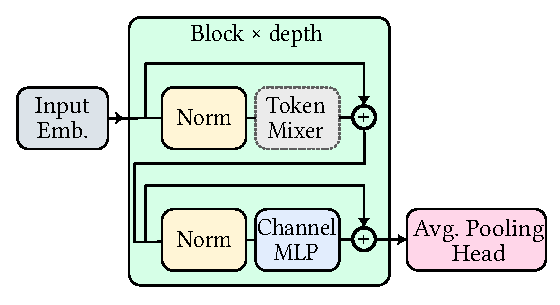
\includegraphics[width=0.8\textwidth]{./architectures/theory/metaformer/metaformer.pdf}}
    \caption{Schematic representation of the \emph{metaformer} concept architecture, adapted to represent the models used in the thesis. 
    The model starts with an input embedding block, that converts the input data into the shape required for the metaformer ($n\times e$) \cite{imageWorth16x16}. This is also the place where possible position encodings are added. 
    After that, the information is passed through \emph{depth} blocks sequentially. 
    A block consists of \emph{norm}, \emph{token mixer}, \emph{residual connection} (+), 
    \emph{norm}, \emph{channel mlp}, \emph{residual connection} (+).
    The model's internal state is brought to the desired output dimension with an \emph{average pooling} operation to get from $n \times e$ to $1 \times e$ and a mlp to get to the desired output dimension $1 \times d_\mathrm{out}$.
    }
    \label{fig:metaformer-architecture}
\end{figure}

It is important to understand, that the \emph{token mixer} is not a predefined element, but a location where multiple different blocks can be inserted. 
This can be seen in \autoref{fig:token-mixer-lineup} for a lineup of some special token mixers. 

The job of the token mixer is to exchange information between the $n$ tokens. 
While the job of processing the information inside a token's embedding (of size $e$) is performed by the \emph{channel mlp}.
The \emph{norm} block is typically a \emph{layer norm}, that is introduced to keep the magnitude of the weights inside a reasonable range.

\begin{figure}[htbp]
    \centering
    \makebox[\textwidth][c]{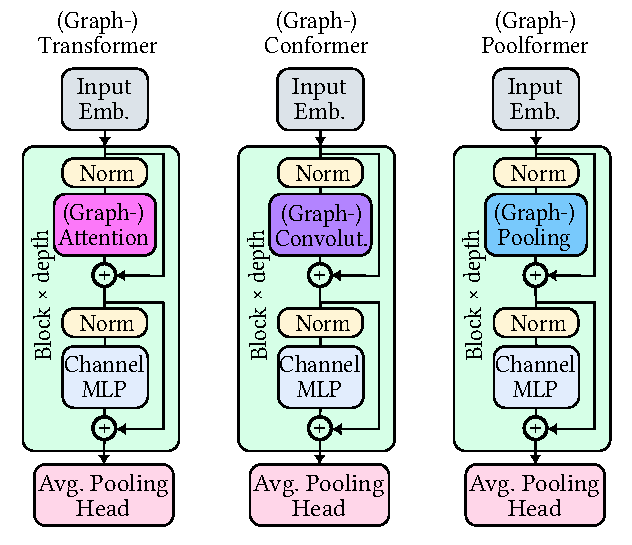
\includegraphics[width=0.7\textwidth]{./architectures/theory/metaformer/token-mixer-lineup.pdf}}
    \caption{Different possible instances of the metaformer architecture presented in \autoref{fig:metaformer-architecture}.
        All structural elements are equivalent to the respective ones in that figure. 
        Only for the placeholder \emph{token mixer}, an \emph{attention-}, \emph{convolution-} and \emph{pooling-}module were inserted, to respectively generate a \emph{transformer}, \emph{conformer} and \emph{poolformer}.
        As different types of convolutions can be defined, the shown models are still technically \emph{classes} of models, but the figure should be enough to convey the concept of token mixer swapping.
        It is important to understand, that the different models' \emph{only difference} is the token mixer they are using.
        The graph versions of the operations are discussed in \autoref{sec:architectures-graphs}.
    }
    \label{fig:token-mixer-lineup}
\end{figure}

The name of the metaformer results from the name of the used token mixer.
A overview is given in \autoref{table:metaformer-names}

\begin{table}[htbp]
    \centering
    \makebox[\textwidth][c]{
        \begin{tabular}{llll} 
            \toprule
            Token mixer & Name & Short & Strict\\  
            \midrule 
            sdp attention & (Vision-)Transformer & TF & yes\\
            attention, masked to nn & Graph (Vision-)Transformer NN & GTF-NN & yes\\
            attention, masked to nnn & Graph (Vision-)Transformer NNN & GTF-NNN & yes\\
            pooling & Poolformer & PF & yes\\
            graph pooling, nn & Poolformer & GPF-NN & yes\\
            graph pooling, nnn & Poolformer & GPF-NNN & yes\\
            full convolution & Conformer & CF & no\\
            symm. convolution, nn & symm. Conformer NN & SCF-NN & no\\
            symm. convolution, nnn & symm. Conformer NNN & SCF-NNN & no\\
            depthw. convolution & dConformer & DCF & yes\\
            symm. depthw. convolution, nn & symm. dConformer NN & SDCF-NN & yes\\
            symm. depthw. convolution, nnn & symm. dConformer NNN & SDCF-NNN & yes\\
            depthw. graph convolution & graph dConformer & GDCF & yes\\
            symm. depthw. graph conv., nn & symm. graph dConformer NN & SGDCF-NN & yes\\
            symm. depthw. graph conv., nnn & symm. graph dConformer NNN & SGDCF-NNN & yes\\
            \bottomrule
        \end{tabular}
    }
    

    \vspace{0.5cm}
    \caption{Overview of the most important metaformer networks. If a network mixes along the \emph{embed dimension} during the token mixing, it is not deemed strict.
    For images or other data stored in rectangular tensor form, the graph- and non-graph-version of poolformer and conformer are equivalent.
    Only the graph variants use the localization bias of data that can not be canonically stored in tensor form. 
    }
    \label{table:metaformer-names}
\end{table}

The table contains an overview of all the metaformer variants that are examined in this thesis.
However other combinations are possible. \emph{GDCF}, \emph{SCF-NN} and \emph{SCF-NNN} are not implemented in the accompanying code \cite{selfPhysics, selfComputerScience}.

How the graph-equivalent modules \emph{graph (depthwise) convolution}, \emph{graph pooling} and \emph{graph masked attention} can be constructed, is described in \autoref{sec:architectures-graphs}.

An exchange of the token mixer module can have different benefits. 
Some can use specially tailored inductive biases to aid the model with its calculation.
Others vary in their storage or computational requirement.
Even more specialized architectures can be attained, if hyperparameters like the embed dimension or the choice of token mixer is varied across the depth of the metaformer. 
Starting with a poolformer of high embed dimension for the first blocks for feature extraction and then reducing the embed dimension to employ a high performance attention module for the final evaluation can result in higher performance than both of the models on their own \cite{metaformerPaper}. 
Hybrid approaches are not discussed in this paper's experiments, but could be a target for further research.

A further modification is shown in \autoref{fig:metaformer-architecture} for the last element.
An \emph{average pooling} operator is used in conjunction with a \emph{MLP} to reshape the output to dimension necessary for the task. 
In the original vision transformers, a \emph{classifier token} was used \cite{dinoPaper}, as this was motivated by the language processing origins of the transformer.
Experiments (during the writing of this thesis) have shown, that the vision transformer performed better on our use cases, if the average pooling head was used, instead of the classifier token. 
Therefore the average pooling head is included as a fixed component of the metaformer architecture in this thesis.

        \FloatBarrier
        \subsection{Graph Architectures}
        \label{sec:architectures-graphs}
        Extending the base metaformer architecture to a graph architecture has three advantages. 
Though a hidden problem will be discussed at the end of this section.

\paragraph{Allowing for the application of established operators} like convolutions and pooling to be used on data that doesn't support encoding in tensor like structures. 
This makes it possible to apply a vast pool of experience and knowledge about convolutional/pooling architectures to graph data, without having to put much thought into inventing new architectures.

\paragraph{Improving performance} of the architecture by introducing new biases.
The \emph{shifted window vision transformer} (swin transformer) \cite{swinTransformerPaper} was able to improve the quality of vision transformers by introducing \emph{non-uniform} blocks that get assembled in a \emph{hierarchical} manner (combining smaller entities to form larger ones and repeating this to form increasingly larger structures).
The swin transformer was not implemented as a graph transformer, because of the already tensor-like structure of images. 
However the good performance of the irregularly merged patches might suggest, that using the powers of the graph networks to \emph{force} irregular interactions may be more efficient, than only hard-encoding a specific lattice structure into the architecture.
Primarily the patch encoder for the lattice input would be a good candidate as a target for further research in that domain.

\paragraph{Becoming encoding independent} as the location in memory and the location in the data structure do not have to be correlated. 
When representing an image in a tensor, the locality information is stored \emph{implicitly} by the location of the values in relation to each other in memory. 
For graph structures, this information is stored \emph{explicitly} in the graphs's edges.
Because of that, the data encoding can be changed and the performance of the graph network is not affected, while changing the positions where data is encoded to, breaks a convolutional filter.
The \autoref{sec:experiments-resiliencylatticeencoding} examines this.\\

A challenge that may present itself, is to what degree a dataset \emph{requires} being encoded as a graph.
Because it is already proven, that for example image classification networks exist, that do not use the inductive biases of locality or translation. 

It probably makes it harder for a neural network to encode a trigonal lattice as a linear array than as a purposefully built graph network with the lattice structure built in.
But as it will become evident in the experiments, it is definitely possible. 
By taking a look at larger lattices, it is obvious they all have a huge degree of periodicity - which is good as that is what defines a lattice.
But at the same time this raises a question: Surely, it is convenient to represent everything as a graph, because they can model most arbitrary relationships (in fact not all relationships \cite{relationalInductiveBiasesAndGraphNetworks}). 
Though they also come with a significant performance overhead when implemented in the current hardware and the methods described in \autoref{sec:architectures-graphs}. 

This poses the question, whether the lattice data experimented on is even \emph{irregular enough} to gain a performance boost from the employment of graph networks.
In follow up research it would therefore definitely be desirable to measure the impact of graph architectures across multiple magnitudes of \glqq irregularity\grqq{} in their structure.

        \FloatBarrier
    \section{Usage of Inductive Biases}
    \label{sec:biases}
    The first set of experiments will be on the image classification task.
The goal will be to compare the architectural advantages and drawbacks between multiple different kinds of metaformers.

Training was be performed on a subset of 100 classes from the \emph{ImageNet} dataset \cite{imagenetDataset}.
The accompanying code to replicate these experiments can be found on GitHub \cite{selfComputerScience}.

The neural networks, as well as the training and evaluation code were written in python.
The \emph{PyTorch} \cite{pytorchGithub} machine learning framework was used as a measure to efficiently define neural networks and lever the computational capabilities of parallelization via GPUs.

The main metaformer model was originally based on the vision transformer found in an implementation of \emph{DINO} \cite{dinoGithub}, was however heavily modified. 
A comparison between the stock DINO model and the modified version will be also performed.
This however is not supposed to be a direct discrediting of any of the models, as their main purposes do not exactly align.
Therefore one or the other may excel in specific tasks.
Also a comparison against a pre-implemented \emph{poolformer} \cite{poolformerGithub} will be performed.

The \emph{einops} package \cite{einopsGithub} is heavily used. It provides tensor operations, configurable with the \emph{Einstein notation} and simplifies the notation and subsequently readability.
Lastly, the implementation of the \emph{positional encoding} is provided by \cite{positionalEncodingGithub}.

        \subsection{Conventional Architectures}
        \label{sec:architectures-biasesnormal}
        Every building block inside a sophisticated neural network contributes to the architecture's inductive bias as a whole, starting from the most basic ones.

\paragraph{Fully connected Layers} have a relatively weak bias, because all inputs relate to all outputs independently \cite{relationalInductiveBiasesAndGraphNetworks}. 
The motivation is to construct a block with relatively high flexibility.
It is barely restricted on the sort of data it can process and can therefore easily be used alongside other computational elements.
In conjunction with a non-linear element (like ReLU), the architecture resembles the structure of the human brain. 
This motivates the assumption, that the element can perform useful computations.
In the field of NQS, the \emph{restricted Boltzmann machine} is often employed.
The RBM basically consists of fully connected layers and can be motivated to be very well suited to model the statistical interactions of many body quantum mechanics \cite{restrictedBoltzmanMachines}. 

\paragraph{Convolutions} work with smaller kernels that get shifted over a larger input space.
This implies the two biases of \emph{locality} and \emph{translation} \cite{relationalInductiveBiasesAndGraphNetworks}.
That means, things close together relate more than things far apart. 
Something that in most cases is very true for images (if a dog's ears are detected, but far apart from each other, this most likely isn't a dog. If they are detected next to each other, this is a good indication for a dog).
Also it doesn't matter, where things are located on the image (a dog in the left corner is a dog in the same way as one on the right).

\paragraph{Symmetric convolutions} have the same biases as their generic counterparts. They however have the additional bias of \emph{only regarding the distance, not the direction}, which implies a kind of \emph{rotational} symmetry.
This helpful, if that data shows dependencies on the proximity of elements in relation to each other. 
The Ising lattices, reviewed in this thesis, have this property. 
If two spins interact or not is only dictated by how close they are, not by the direction one is from the other.

\paragraph{Depthwise (separable) convolutions} were introduced by research on how to efficiently reduce network size \cite{mobileNetPaper}.
Their bias is, that interaction between values of one channel (for example one color channel in the case of rgb-images) can be computed independent and then only combined in a second step.
This makes sense, as there is already quite a lot of information inside one color channel. 
And as extracting the information per channel before comparing across channels saves a lot of computational resources, this is a logical step to take.
Also it should in most cases be possible to recognize e.g. a dogs shape only from one color channel. 
Therefore checking for a shape in all channels separately and then comparing seems easier than forcefully training to assemble shapes across channels.

\paragraph{Recurrent layers} are used a lot in translation tasks and video analysis, because of their \emph{time invariance} \cite{relationalInductiveBiasesAndGraphNetworks}. 
These would likely be very powerful for investigating the development of a quantum system over time. 
As this thesis focuses on stationary problems, recurrency is not used.

\paragraph{Residual connections} are used for a value in a calculation to be able to bypass a block completely.
The metaformer architecture in \autoref{fig:metaformer-architecture} includes residual connections as an important part.
They are motivated by the bias, that it is simpler to zero out an element in a machine learning architecture, than to learn the \emph{identity operation}. 
So if the network recognizes a block does more harm than good in terms of getting the correct solution, it can easily be bypassed by zeroing the block's inputs and using the residual connection. 
At the same time it is unlikely for the element to hurt, as basically each building block can be trained to learn the identity operation, but if a block is not needed it only generates training errors, no additional value \cite{deepResidualLearningForImageRecognition}.
As this element is very likely to be useful in deep networks like metaformers, all the architectures in the performed experiments use residual connections.

\paragraph{Pooling operators} have many similarities to convolutions. They however have the added bias, that the relation does not even depend on the position of a value inside the kernels influence. 
It solely depends on the relative values. 
If this true for the data and the answer really only depends on for example the \emph{average} of the values, this module greatly increases computational speed and decreases the required memory.
This on the other hand allows for evaluating larger/deeper networks which may be desirable.
        \FloatBarrier
        \subsection{Metaformer Architectures}
        \label{sec:architectures-biasesmetaformer}
        The research performed in the \emph{MetaFormer is Actually What You Need for Vision} paper \cite{metaformerPaper} has been very influential in advertising the potential of the \emph{transformer architecture}.
Previously, the model's huge performance was attributed to the attention module, that was introduced in the previous \autoref{sec:architectures-attention}. 
By building alternative models - that shared the structure of the transformer in everything but the attention module - the researchers were able to show that the credit belongs to the structural architecture.

A new class of models, dubbed \emph{metaformer} by the authors, was introduced. 
The architecture's good performance can be motivated through its inductive biases, which will be addressed in \autoref{sec:architectures-biasesmetaformer}.
The following section is only supposed to introduce the naming scheme that is going to be used in the later parts of this thesis.

The general structure of the metaformer can be seen in \autoref{fig:metaformer-architecture}.

\begin{figure}[htbp]
    \centering
    \makebox[\textwidth][c]{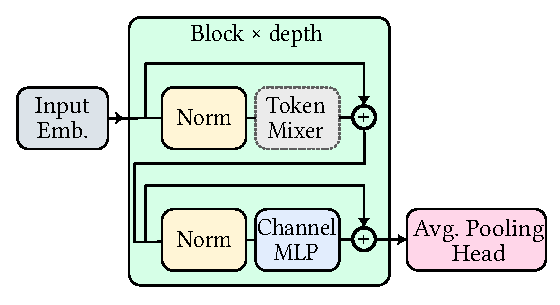
\includegraphics[width=0.8\textwidth]{./architectures/theory/metaformer/metaformer.pdf}}
    \caption{Schematic representation of the \emph{metaformer} concept architecture, adapted to represent the models used in the thesis. 
    The model starts with an input embedding block, that converts the input data into the shape required for the metaformer ($n\times e$) \cite{imageWorth16x16}. This is also the place where possible position encodings are added. 
    After that, the information is passed through \emph{depth} blocks sequentially. 
    A block consists of \emph{norm}, \emph{token mixer}, \emph{residual connection} (+), 
    \emph{norm}, \emph{channel mlp}, \emph{residual connection} (+).
    The model's internal state is brought to the desired output dimension with an \emph{average pooling} operation to get from $n \times e$ to $1 \times e$ and a mlp to get to the desired output dimension $1 \times d_\mathrm{out}$.
    }
    \label{fig:metaformer-architecture}
\end{figure}

It is important to understand, that the \emph{token mixer} is not a predefined element, but a location where multiple different blocks can be inserted. 
This can be seen in \autoref{fig:token-mixer-lineup} for a lineup of some special token mixers. 

The job of the token mixer is to exchange information between the $n$ tokens. 
While the job of processing the information inside a token's embedding (of size $e$) is performed by the \emph{channel mlp}.
The \emph{norm} block is typically a \emph{layer norm}, that is introduced to keep the magnitude of the weights inside a reasonable range.

\begin{figure}[htbp]
    \centering
    \makebox[\textwidth][c]{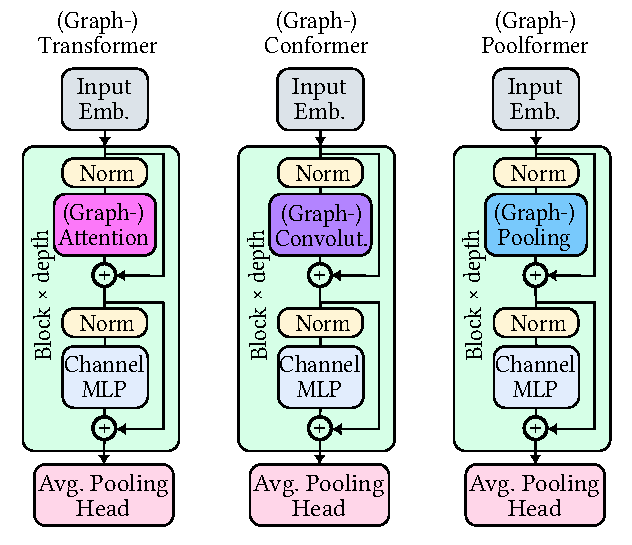
\includegraphics[width=0.7\textwidth]{./architectures/theory/metaformer/token-mixer-lineup.pdf}}
    \caption{Different possible instances of the metaformer architecture presented in \autoref{fig:metaformer-architecture}.
        All structural elements are equivalent to the respective ones in that figure. 
        Only for the placeholder \emph{token mixer}, an \emph{attention-}, \emph{convolution-} and \emph{pooling-}module were inserted, to respectively generate a \emph{transformer}, \emph{conformer} and \emph{poolformer}.
        As different types of convolutions can be defined, the shown models are still technically \emph{classes} of models, but the figure should be enough to convey the concept of token mixer swapping.
        It is important to understand, that the different models' \emph{only difference} is the token mixer they are using.
        The graph versions of the operations are discussed in \autoref{sec:architectures-graphs}.
    }
    \label{fig:token-mixer-lineup}
\end{figure}

The name of the metaformer results from the name of the used token mixer.
A overview is given in \autoref{table:metaformer-names}

\begin{table}[htbp]
    \centering
    \makebox[\textwidth][c]{
        \begin{tabular}{llll} 
            \toprule
            Token mixer & Name & Short & Strict\\  
            \midrule 
            sdp attention & (Vision-)Transformer & TF & yes\\
            attention, masked to nn & Graph (Vision-)Transformer NN & GTF-NN & yes\\
            attention, masked to nnn & Graph (Vision-)Transformer NNN & GTF-NNN & yes\\
            pooling & Poolformer & PF & yes\\
            graph pooling, nn & Poolformer & GPF-NN & yes\\
            graph pooling, nnn & Poolformer & GPF-NNN & yes\\
            full convolution & Conformer & CF & no\\
            symm. convolution, nn & symm. Conformer NN & SCF-NN & no\\
            symm. convolution, nnn & symm. Conformer NNN & SCF-NNN & no\\
            depthw. convolution & dConformer & DCF & yes\\
            symm. depthw. convolution, nn & symm. dConformer NN & SDCF-NN & yes\\
            symm. depthw. convolution, nnn & symm. dConformer NNN & SDCF-NNN & yes\\
            depthw. graph convolution & graph dConformer & GDCF & yes\\
            symm. depthw. graph conv., nn & symm. graph dConformer NN & SGDCF-NN & yes\\
            symm. depthw. graph conv., nnn & symm. graph dConformer NNN & SGDCF-NNN & yes\\
            \bottomrule
        \end{tabular}
    }
    

    \vspace{0.5cm}
    \caption{Overview of the most important metaformer networks. If a network mixes along the \emph{embed dimension} during the token mixing, it is not deemed strict.
    For images or other data stored in rectangular tensor form, the graph- and non-graph-version of poolformer and conformer are equivalent.
    Only the graph variants use the localization bias of data that can not be canonically stored in tensor form. 
    }
    \label{table:metaformer-names}
\end{table}

The table contains an overview of all the metaformer variants that are examined in this thesis.
However other combinations are possible. \emph{GDCF}, \emph{SCF-NN} and \emph{SCF-NNN} are not implemented in the accompanying code \cite{selfPhysics, selfComputerScience}.

How the graph-equivalent modules \emph{graph (depthwise) convolution}, \emph{graph pooling} and \emph{graph masked attention} can be constructed, is described in \autoref{sec:architectures-graphs}.

An exchange of the token mixer module can have different benefits. 
Some can use specially tailored inductive biases to aid the model with its calculation.
Others vary in their storage or computational requirement.
Even more specialized architectures can be attained, if hyperparameters like the embed dimension or the choice of token mixer is varied across the depth of the metaformer. 
Starting with a poolformer of high embed dimension for the first blocks for feature extraction and then reducing the embed dimension to employ a high performance attention module for the final evaluation can result in higher performance than both of the models on their own \cite{metaformerPaper}. 
Hybrid approaches are not discussed in this paper's experiments, but could be a target for further research.

A further modification is shown in \autoref{fig:metaformer-architecture} for the last element.
An \emph{average pooling} operator is used in conjunction with a \emph{MLP} to reshape the output to dimension necessary for the task. 
In the original vision transformers, a \emph{classifier token} was used \cite{dinoPaper}, as this was motivated by the language processing origins of the transformer.
Experiments (during the writing of this thesis) have shown, that the vision transformer performed better on our use cases, if the average pooling head was used, instead of the classifier token. 
Therefore the average pooling head is included as a fixed component of the metaformer architecture in this thesis.

        \FloatBarrier
        \subsection{Graph Architectures}
        \label{sec:architectures-biasesgraph}
        Extending the base metaformer architecture to a graph architecture has three advantages. 
Though a hidden problem will be discussed at the end of this section.

\paragraph{Allowing for the application of established operators} like convolutions and pooling to be used on data that doesn't support encoding in tensor like structures. 
This makes it possible to apply a vast pool of experience and knowledge about convolutional/pooling architectures to graph data, without having to put much thought into inventing new architectures.

\paragraph{Improving performance} of the architecture by introducing new biases.
The \emph{shifted window vision transformer} (swin transformer) \cite{swinTransformerPaper} was able to improve the quality of vision transformers by introducing \emph{non-uniform} blocks that get assembled in a \emph{hierarchical} manner (combining smaller entities to form larger ones and repeating this to form increasingly larger structures).
The swin transformer was not implemented as a graph transformer, because of the already tensor-like structure of images. 
However the good performance of the irregularly merged patches might suggest, that using the powers of the graph networks to \emph{force} irregular interactions may be more efficient, than only hard-encoding a specific lattice structure into the architecture.
Primarily the patch encoder for the lattice input would be a good candidate as a target for further research in that domain.

\paragraph{Becoming encoding independent} as the location in memory and the location in the data structure do not have to be correlated. 
When representing an image in a tensor, the locality information is stored \emph{implicitly} by the location of the values in relation to each other in memory. 
For graph structures, this information is stored \emph{explicitly} in the graphs's edges.
Because of that, the data encoding can be changed and the performance of the graph network is not affected, while changing the positions where data is encoded to, breaks a convolutional filter.
The \autoref{sec:experiments-resiliencylatticeencoding} examines this.\\

A challenge that may present itself, is to what degree a dataset \emph{requires} being encoded as a graph.
Because it is already proven, that for example image classification networks exist, that do not use the inductive biases of locality or translation. 

It probably makes it harder for a neural network to encode a trigonal lattice as a linear array than as a purposefully built graph network with the lattice structure built in.
But as it will become evident in the experiments, it is definitely possible. 
By taking a look at larger lattices, it is obvious they all have a huge degree of periodicity - which is good as that is what defines a lattice.
But at the same time this raises a question: Surely, it is convenient to represent everything as a graph, because they can model most arbitrary relationships (in fact not all relationships \cite{relationalInductiveBiasesAndGraphNetworks}). 
Though they also come with a significant performance overhead when implemented in the current hardware and the methods described in \autoref{sec:architectures-graphs}. 

This poses the question, whether the lattice data experimented on is even \emph{irregular enough} to gain a performance boost from the employment of graph networks.
In follow up research it would therefore definitely be desirable to measure the impact of graph architectures across multiple magnitudes of \glqq irregularity\grqq{} in their structure.

        \FloatBarrier

\chapter{Experiments and their Results}
\label{sec:experiments}
    \section{Metaformer in Image Classification}
    \label{sec:experiments-image-classification}
    The first set of experiments will be on the image classification task.
The goal will be to compare the architectural advantages and drawbacks between multiple different kinds of metaformers.

Training was be performed on a subset of 100 classes from the \emph{ImageNet} dataset \cite{imagenetDataset}.
The accompanying code to replicate these experiments can be found on GitHub \cite{selfComputerScience}.

The neural networks, as well as the training and evaluation code were written in python.
The \emph{PyTorch} \cite{pytorchGithub} machine learning framework was used as a measure to efficiently define neural networks and lever the computational capabilities of parallelization via GPUs.

The main metaformer model was originally based on the vision transformer found in an implementation of \emph{DINO} \cite{dinoGithub}, was however heavily modified. 
A comparison between the stock DINO model and the modified version will be also performed.
This however is not supposed to be a direct discrediting of any of the models, as their main purposes do not exactly align.
Therefore one or the other may excel in specific tasks.
Also a comparison against a pre-implemented \emph{poolformer} \cite{poolformerGithub} will be performed.

The \emph{einops} package \cite{einopsGithub} is heavily used. It provides tensor operations, configurable with the \emph{Einstein notation} and simplifies the notation and subsequently readability.
Lastly, the implementation of the \emph{positional encoding} is provided by \cite{positionalEncodingGithub}.

        \subsection{Training Settings}
        \label{sec:experiments-trainingsettings}
        The comparison of different architectures in a fair manner is not trivial to do.
Because it is possible that the performance of an architecture is highly dependent on the used hyperparameters, for a fair comparison it would be necessary to optimize the hyperparameters for every architecture and only compare the top scoring results.
As performing training runs for this thesis takes durations ranging from \SI[]{30}[]{\minute} to \SI[]{12}[]{\hour}, it is not feasible to run the powerset of hyperparameter combinations and choose only the best.
Even with the resources provided by Augsburg University to calculate a higher number of runs than were ever possible on only my local machines, investing months into these calculations is neither possible, nor sensible.

Therefore an informed pre-selection of likely interesting runs had to be chosen beforehand.
Helpful in this manner were the previous experiences by other researchers. 
The metaformer's hyperparameters \emph{image size}, \emph{number of heads}, \emph{patch size}, \emph{embed dimension}, \emph{depth} and \emph{mlp ratio} have been chosen as the same values, the \emph{DINO tiny} model was implemented in \cite{dinoGithub}. As the transformer in the DINO paper \cite{dinoPaper} was a structural template for this metaformer, selecting the smallest model from their lineup made it possible to perform as many comparisons as possible with limited resources.

In order to understand what is measured, a full overview of the recorded parameters is presented in \autoref{fig:comparison-recorded-values}.

\begin{figure}[htbp]
    \centering
    \makebox[\textwidth][c]{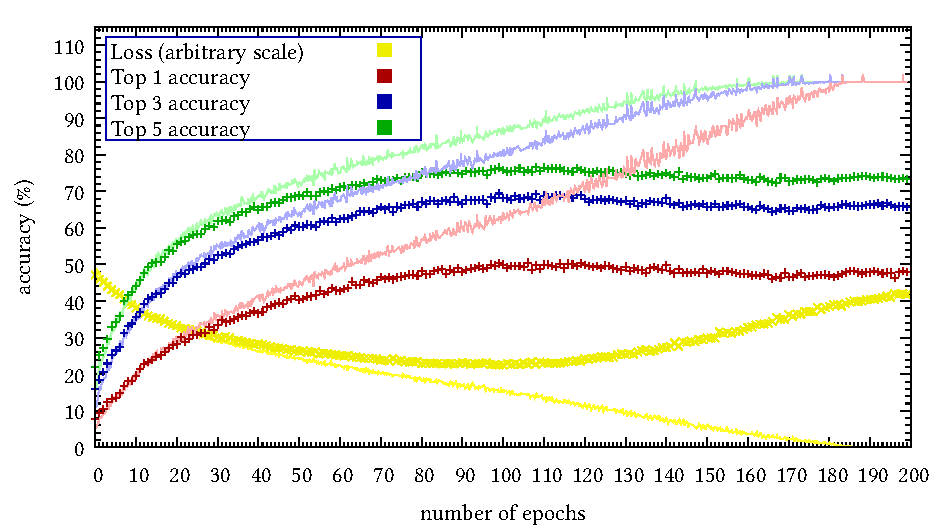
\includegraphics[width=1.1\textwidth]{./experiments/image-classification/training-settings/metrics/metrics.pdf}}
    \caption{Graphic depiction of all recorded metrics for the image classification task.
    The data is from a \emph{CF} metaformer and has been selected because it clearly shows the expected behavior of convergence.
    The \emph{accuracy} (\autoref{sec:theory-imageclassification}) and \emph{loss} (\autoref{sec:theory-neuralnetworktraining}) are depicted. 
    The results from \emph{testing} the model on the validation set are depicted as individual data points and colored dark. 
    The data collected during the \emph{training} calculations are colored in the corresponding color, but shaded more brightly. The training data is plotted as a smoothed line, to allow for a more pleasant viewing experience.
    The loss data is scaled arbitrarily to fit into the graph, as the absolute values are not relevant. }
    \label{fig:comparison-recorded-values}
\end{figure}

All the runs share a few key similarities. Because of that, the full data for one run is only shown once. 
Later figures will leave out most of the metrics, because they are almost completely redundant.

The model training always follows the same default structure: The accuracy starts low and the loss starts at a high value.
This is expected as in the beginning the model only guesses randomly. 
Therefore a top-1-accuracy should start at around \SI[]{1}[]{\percent} for a classification task of 100 classes.
It can be lower or higher depending on random chance, but in general it holds for very early values. 
As the results improve very rapidly in the first few epochs, this can not be seen in the charts for most runs.
Also it should be noted, that the first recorded \emph{test} data point is calculated \emph{after} the first epoch. 
The model therefore is already advanced and no longer random. 
This explains, why the curves start higher than expected.

A shared trend for all datasets is, that the top-3-accuracy lies above the top-1-accuracy and the top-5-accuracy above both. 
This is necessary, because if a model classifies the correct answer among the best three highest rated answers, it automatically has also classified it among the top five. 
Because of that only the performance for the top class predictions will be shown, as the other metrics provide not much  additional insight into the comparison between architectures.

It can also be observed, that the \emph{test} accuracy rises at first, then plateaus and finally falls off.
The \emph{training} accuracy however constantly rises and can even hit \SI[]{100}[]{\percent}.
This can be explained by overfitting (\autoref{sec:theory-neuralnetworktraining}).
As explained, the amount of training data is limited. 
Therefore the model is presented with the same image many times. 
As it is allowed to adjust its weights based on the training data, it is possible for it to \glqq remember\grqq{} all solutions.
As can be clearly seen by the descending test performance after a specific point, doing so is not helpful for classifying unseen images.
Overfitting can be counteracted by setting so called \emph{dropout} connections/weights.
By randomly setting weights to zero, the model is always restricted to a subset of its weights and therefore has to develop a more robust internal representation. This reduces/delays the overfitting behavior.

The goal however is to detect differences in the architectural design. 
Thus it is important to be able to differentiate whether a poolformer is inherently more robust to overfitting than a conformer or the other way around. Because of that the dropout always is set to zero.

Subsequently, all models were trained to the point of overfitting. 
If statements about the accuracy of a model are made, the highest value of the \emph{test accuracy} is presented.
For \autoref{fig:comparison-recorded-values} this is at epoch 106.
It can be noted, that this is also the point, at which the train loss starts to rise again.
As explained previously, the loss is a measure of model's performance. 
The smaller the loss, the better the representation. 
If the test loss is rising and the train loss is still falling, this is a clear indication for the model being in the process of overfitting. 
This can be summarized to the rule, that all models were trained to the point, where either the test accuracy was noticeably dropping or the test loss was noticeably rising.
If accuracies are plotted, that have no clearly visible drop-off at the end, this is because the overfitting could be recognized in trend of the loss. 
Calculations then often were aborted to save resources.

\begin{figure}[htbp]
    \centering
    \makebox[\textwidth][c]{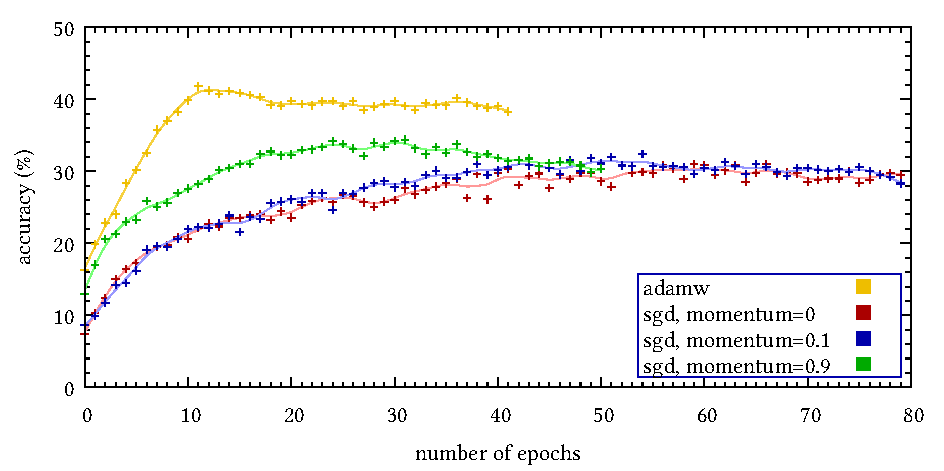
\includegraphics[width=1.1\textwidth]{./experiments/image-classification/training-settings/optimizer/optimizer.pdf}}
    \caption{Comparison of the top-1-accuracy for training a modified DINO tiny transformer.
    Different optimizer algorithms are used for the backpropagation.
    The training accuracy is pictured, the lighter colored lines are interpolations of the data with square splines. 
    This is supposed to make the differentiation of the red and blue curve easier.
    }
    \label{fig:optimizer}
\end{figure}

\autoref{fig:optimizer} shows a subset of the experiments performed to choose an appropriate \emph{optimizer} and learning rate.
It can be easily seen, that the choice of optimization algorithm influences the speed of convergence, as well as the maximum performance of the networks.
The \emph{adamw} \cite{adamwOptimizer} optimizer performed best in both of these metrics.
The established \emph{stochastic gradient descent} update algorithm scored a between \SIrange[]{10}{15}{\percent} worse test accuracy, as well as a two to four times slower rate of convergence in relation to the number of epochs.

Increasing the momentum value comes with no additional costs or drawbacks, however it leads to overall better performing models, that converge faster \cite{momentum}.
Because of that \SI{0.9}{} was chosen as the momentum value for the sgd in all subsequent runs.

In literature, multiple comparisons between the different optimization mechanisms have been performed \cite{sgdOrAdamw}.
Though the adamw optimizer performed better, the update procedure is also more expensive, in particular requiring more memory.
Because of that, the batch size could not be set to 128 (like for the sgd optimizer), but had to be reduced to 64, as the available GPU memory was quite limited at the start of the experiments.
At the same time, the sgd algorithm produced more consistent trends with less abrupt changes.
In order to again choose reliable comparability above maximum performance, only the sgd optimizer is used in subsequent image recognition experiments. 

All of the optimizers use a constant \emph{learning rate} of \SI[]{0.001}{}{}.
        \FloatBarrier
        \subsection{Importance of Positional Encoding}
        \label{sec:experiments-positionalencoding}
        Just as described in \autoref{sec:architectures-attention}, the transformer architecture's performance can be improved by providing it \emph{positional encoding} (pe) information.
While with convolutions and pooling, identical patches at different locations can be distinguished, in the attention mechanism they can't.
Adding pe should (end does) improve this.

The question is, whether the \emph{masked} attention, that uses the graph information to confine the transformer to only its local neighborhood, also requires pe or not. 
And if efficient training requires pe, what type works best.

\begin{figure}[htbp]
    \centering
    \makebox[\textwidth][c]{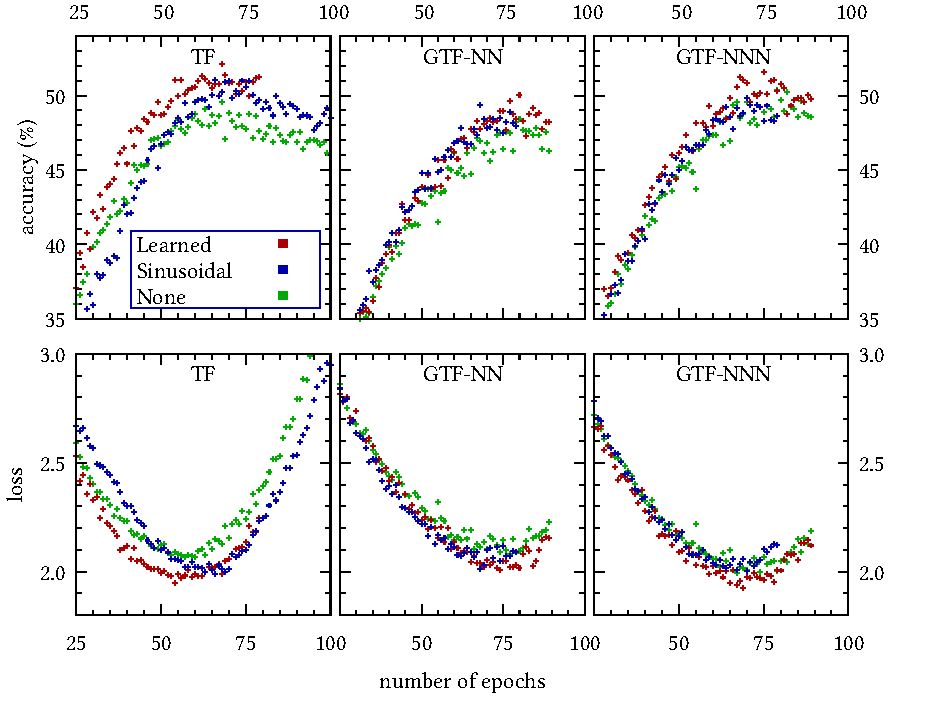
\includegraphics[width=1.1\textwidth]{./experiments/image-classification/positional-encoding/pe-comparison/pe-comparison.pdf}}
    \caption{Visualization of the training attention and loss metrics for three different models. \emph{TF}, \emph{GTF-NN} and \emph{GTF-NNN}.
    Only part of the full training is shown. 
    Each model was trained once with \emph{sinusoidal} pe, \emph{learned} pe and \emph{without} any additional pe.
    Apart from that all hyperparameters are kept static.
    }
    \label{fig:positional-encoding-training}
\end{figure}

The experiments are visualized in \autoref{fig:positional-encoding-training}.
It can be clearly seen, that the different architectures react differently to the types of pe.

The data clearly shows benefits in employing pe. 
All models show an increase in accuracy of about \SIrange[]{3}{4}{\percent}. 
This is less than the difference between some of the other token mixing elements, but still a significant margin in comparison to the absolute performance.
As adding pe is rather cheap, the employment of this strategy can definitely be useful:
Both types of pe are only added at the start of the calculation.
Therefore the cost is not dependent on the depth or type of token-mixer.
Calculating sinusoidal pe can theoretically be done once and the result can be cached, rendering it basically instantaneous to employ and of no negative computational impact. Furthermore it is resolution independent, as the sinus curves can later be sampled with a smaller interval in order to increase network resolution retrospectively.
Learned sinusoidal encodings on the other hand require a backwards propagation of error values into the encoding weights.
This requires additional computation and storage space, as well as providing no obvious way to update the encoding resolution after the fact.

The pure transformer definitely performs best with a learned pe. 
Not only is the overall accuracy higher ($\approx \SI[]{1.5}[]{\percent}$), but loss-minimum is reached about 12 epochs earlier - a huge potential reduction in necessary computation.

The GTF-NN model shows less benefit from applying pe.
This makes sense, as by design the number of attention targets is intentionally very limited. 
Sinusoidal pe and learned pe perform very similar, with sinusoidal pe converging ever so slightly faster than learned.
It should be noted though, that the sample size is too limited to draw definite conclusions from this tiny difference.

In the GTF-NNN, the learned pe outperforms the sinusoidal one, taking about 5 epochs longer to converge, but accomplishing an about \SI[]{2}{\percent} better accuracy.

To summarize, the pe can definitely improve the performance of an attention based neural network. 
That this was the case for normal attention was already know \cite{attentionIsAllYouNeed, imageWorth16x16}. 
Now this small scale experiment shows, that the correlation can hold true for the attention mechanism with graph-limited influence.

A challenge in more complex graph structures is undoubtably the definition of suitable pes, as the canonical sinusoidal encoding is not  extendable to irregular graphs.
The learned pe would probably constitute the easiest and best solution, but comes with a computational overhead both in terms of the cost of one epoch, as well as the speed of convergence (needed number of epochs until converged).

In the ground state search task, no positional encoding is applied. 
This could be a target for future research, especially on highly irregular graphs.
        \FloatBarrier
        \subsection{Comparison of different Token Mixers}
        \label{sec:experiments-tokenmixers}
        In \autoref{sec:architectures-graphs} it was established, that for tensor-like data, \emph{convolutions} and \emph{graph-convolutions} are exactly the same thing, only calculated differently.

This thesis was validated experimentally and is visualized in \autoref{fig:graph-convolution-works}.

\begin{figure}[htbp]
    \centering
    \makebox[\textwidth][c]{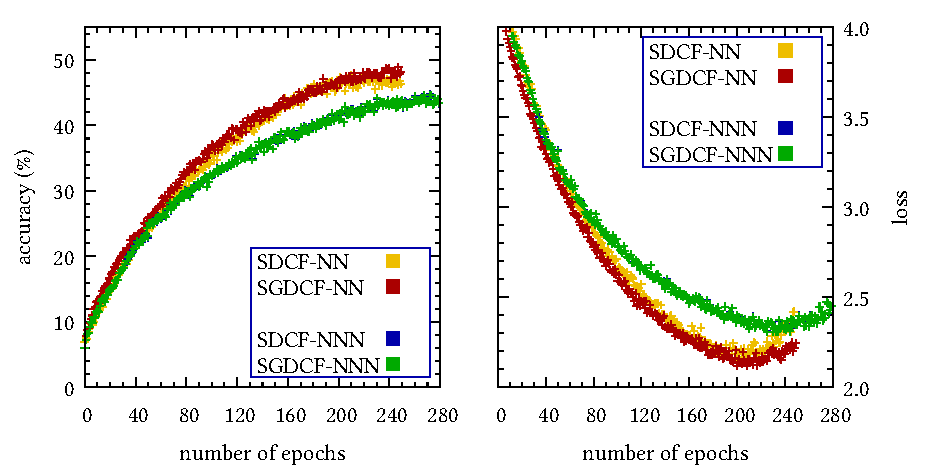
\includegraphics[width=1.1\textwidth]{./experiments/image-classification/comparison-token-mixers/graph-conv/graph-conv.pdf}}
    \caption{
        Comparison of the behavior of the traditional convolution based conformers (yellow and blue) to the graph based ones for image training data.
        The Blue and the green curve are completely identical (but calculated by optimizing different models), therefore blue is not visible.
        The reason, why the red and yellow curve are not also identical is due to different uses of the random number generator.
    }
    \label{fig:graph-convolution-works}
\end{figure}

The data clearly shows, that the implementations of SDCF-NNN and SGDCF-NNN behave exactly identical, even though they compute the path interactions with different operations, as they are mathematically identical.

It is natural to expect, that SDCF-NN and SGDCF-NN behave likewise, but slight differences in the data of theses two be observed.
This is because of the pseudo random number generator used in PyTorch.
The implementation of the graph-convolution (\emph{GraphMaskConvolution} in \cite{selfComputerScience} \filepath{/models/metaformer.py}) and the conventional-convolution (\emph{SymmDepthSepConv2d} in \cite{selfComputerScience} \filepath{/models/helpers/SymmConv2d.py}) query the random number generator a different number of times, because the graph implementation always allocates ($3 \cdot \mathrm{channels}$) weights and the conventional implementation only allocates ($2 \cdot \mathrm{channels}$) weights for nn interactions and ($3 \cdot \mathrm{channels}$) for nnn.
This causes the random number generator to drift apart and produces a propagating difference in the calculations \emph{only} for nn and not for nnn.

While this is a fixable flaw of the implementation, it clearly shows that the graph and non-graph implementations are behaving similar, even if the starting conditions are non-equivalent.
The comparison among the whole set of metaformers will emphasize how similar these two curves really are.

This proves, that convolutions can directly be translated into a graph context and motivates their function on non-tensor-like data structures.

        \FloatBarrier
        \subsection{Efficiency of Graph Attention}
        \label{sec:experiments-efficiency-graphs}
        As a closing argument to the first set of experiments, the efficiency of graph masked attention will be discussed.

While the experimental results in \autoref{sec:experiments-tokenmixers} (especially \autoref{table:overall-comparison-data}) showed a performance lead for the attention based transformers, as stated this operation is still comparably expensive.
The \emph{GTF} architecture had by far the longest training time per epoch of the examined models.
This is because of the inherent cost of the \emph{attention} operation that scales $\propto \mathcal{O}(n^2)$ with the number of nodes (in case of images, the number of patches) $n$, onto which the costs for masking the not required attention connections are added (also $\propto \mathcal{O}(n^2)$).

This doesn't have to be the case though, it merely is a result of the chosen computational algorithm: 
\begin{enumerate}
    \setlength\itemsep{-0.5em}
    \item calculate \emph{all} interactions from every node with every node
    \item mask and scale only the interactions belonging to 
        \begin{itemize}
            \setlength\itemsep{-0.5em}
            \item the node itself
            \item the nearest neighbors
            \item the next nearest neighbors
        \end{itemize}
    \item add all scaled interactions
    \item replace all zeros with $-\infty$ to make them vanish in the softmax
\end{enumerate}

Looking at this again, it is clear a great number of computations is wasted. 
Every entry of the outer product that is no self, nn- or nnn-interaction \emph{will} get overwritten with $-\infty$.
Also all entries that contain $-\infty$ get passed through softmax, \emph{even though} is is clear beforehand that they will not contribute anything.

Each node has (depending on the chosen interaction paradigm) only a constant number $c$ of nodes it is going to interact with.
For large Graphs, this $c << n$. 
With that in mind, the calculation really should have the complexity $\mathcal{O}(c \cdot n) \rightarrow \mathcal{O}(n)$, because for each of the $n$ nodes, only $c$ interactions should have to be calculated and passed through the softmax.

As the code in the implementation makes use of GPUs to accelerate the computation, it is still faster to calculate the unused connections and \glqq throw\grqq{} them away shortly after.
Because this harnesses the GPUs, highly optimized implementation of operations like matrix multiplication.

But through implementing the linear time calculation efficiently and compiling it to the GPU instructionset, a massive speedup could be achieved. 
This would bring in the benefits of the attention operation, but get rid of the $\mathcal{O}(n^2)$ complexity problem.
While not having the full attention at ones disposal, the graph masked attention still is absolutely competitive for some use cases (\autoref{table:overall-comparison-data}).

An even greater speedup could be achieved by implementing the described algorithm directly in hardware.
While the current demand for graph attention calculation may not yet be high enough to justify this, future developments could easily make investing in this technology worthwhile.

        \FloatBarrier

    \section{Metaformer in Ground State Search}
    \label{sec:experiments-ground-state-search}
    The first set of experiments will be on the image classification task.
The goal will be to compare the architectural advantages and drawbacks between multiple different kinds of metaformers.

Training was be performed on a subset of 100 classes from the \emph{ImageNet} dataset \cite{imagenetDataset}.
The accompanying code to replicate these experiments can be found on GitHub \cite{selfComputerScience}.

The neural networks, as well as the training and evaluation code were written in python.
The \emph{PyTorch} \cite{pytorchGithub} machine learning framework was used as a measure to efficiently define neural networks and lever the computational capabilities of parallelization via GPUs.

The main metaformer model was originally based on the vision transformer found in an implementation of \emph{DINO} \cite{dinoGithub}, was however heavily modified. 
A comparison between the stock DINO model and the modified version will be also performed.
This however is not supposed to be a direct discrediting of any of the models, as their main purposes do not exactly align.
Therefore one or the other may excel in specific tasks.
Also a comparison against a pre-implemented \emph{poolformer} \cite{poolformerGithub} will be performed.

The \emph{einops} package \cite{einopsGithub} is heavily used. It provides tensor operations, configurable with the \emph{Einstein notation} and simplifies the notation and subsequently readability.
Lastly, the implementation of the \emph{positional encoding} is provided by \cite{positionalEncodingGithub}.

        \subsection{Comparison to established Architectures}
        \label{sec:experiments-comparisontoestablished}
        % TODO


\begin{figure}[htbp]
    \centering
    \makebox[\textwidth][c]{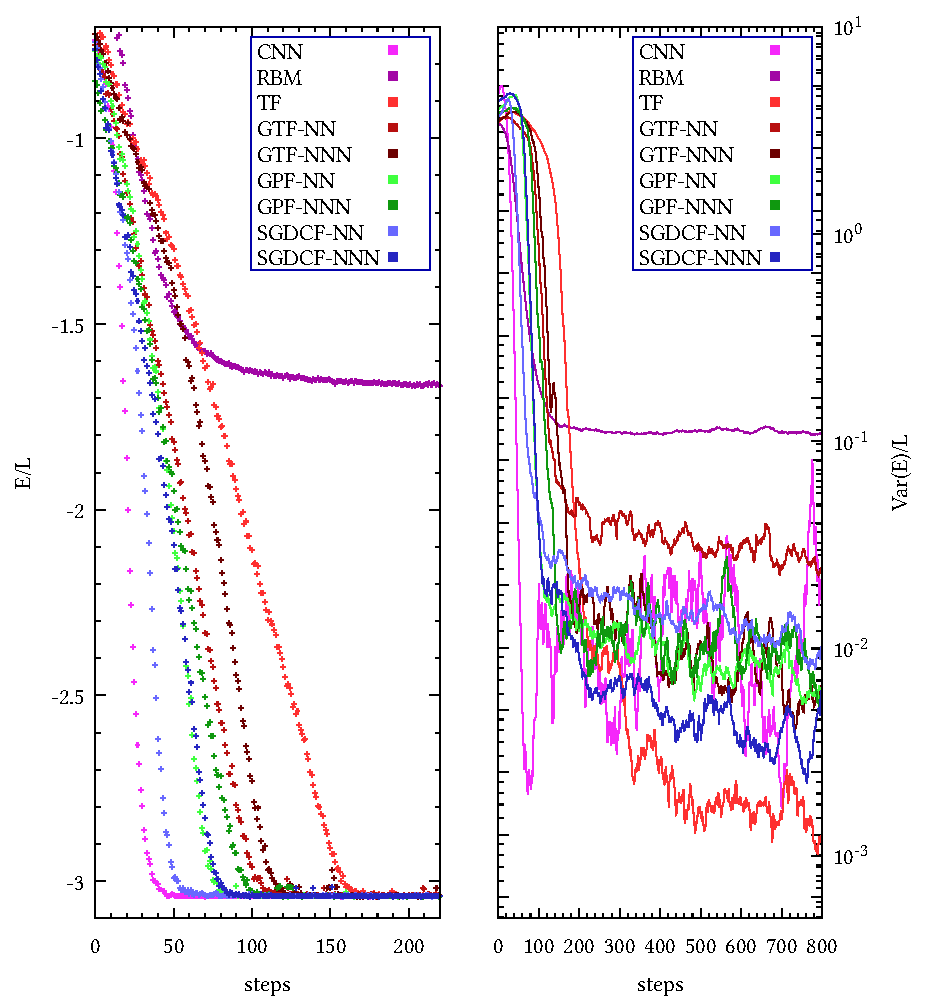
\includegraphics[width=1.1\textwidth]{./experiments/ground-state-search/comparison-established/architecture-comparison/architecture-comparison.pdf}}
    \caption{A comparison of different established and novel neural network architectures used as NQS in a ground state search.
        The calculations were performed for a 2D-trigonal\_hexagonal lattice of size 3 (37 lattice sites).
        The lattice is periodic and the encoding is set to be random.
        The models were configured to be as similar as possible in terms of the number of trainable weights.
        The \emph{CNN} was set to have 16 channels ($\stackrel{\wedge}{=}$ 592 weights), The \emph{RBM} was set have 8 hidden layers ($\stackrel{\wedge}{=}$ 592 weights). 
        All metaformers were set to a depth of 2, and a mlp-ratio of 2.
        The poolformers have an embed-dimension of 7 ($\stackrel{\wedge}{=}$ 560 weights for \emph{GPF-NN} and 602 for \emph{GPF-NNN}).
        The conformers also have their embed dimension set to 7 ($\stackrel{\wedge}{=}$ 602 weights for \emph{SGDCF-NN} and 644 for \emph{SGDCF-NNN}).
        Finally the transformers are set to have an embed-dimension of 5 ($\stackrel{\wedge}{=}$ 530 weights for \emph{TF}, 566 weights for \emph{GTF-NN} and 596 weights for \emph{GTF-NN}). 
        Important to notice are the different scales of the x-axes, the energy per site is only shown until step 200, because after that nothing of interest happens. The variance of the energy is shown until step 800.  
        The variance data is interpolated with a moving average in the logarithmic scale of width 35 steps.
    }
    \label{fig:gss-architectures-comp}
\end{figure}
        \FloatBarrier
        \subsection{Resiliency to the Choice of Lattice Encoding}
        \label{sec:experiments-resiliencylatticeencoding}
        % TODO

\begin{figure}[htbp]
    \centering
    \makebox[\textwidth][c]{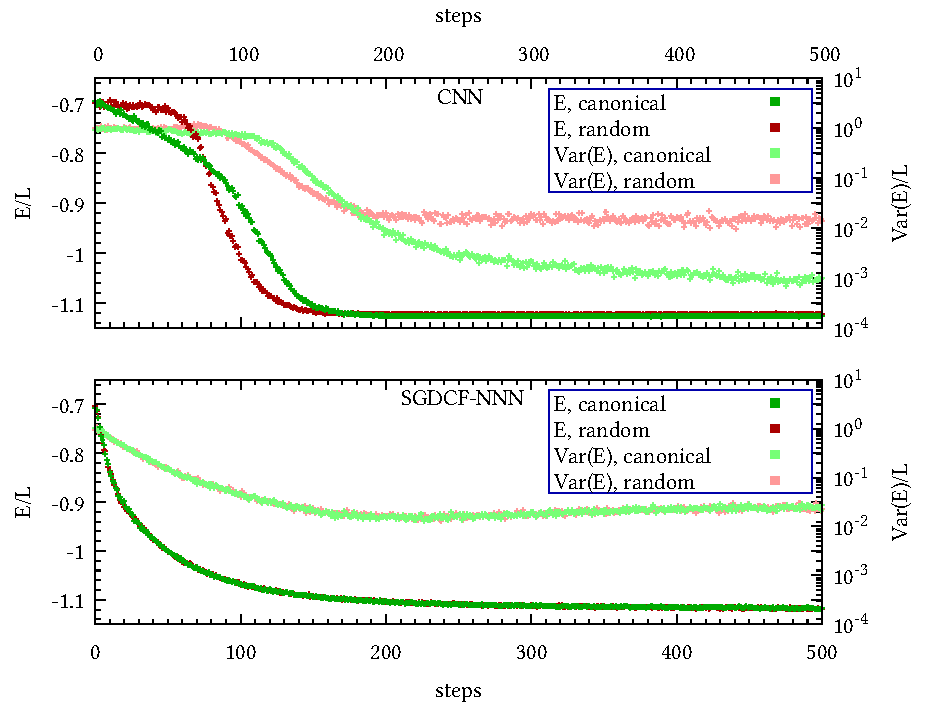
\includegraphics[width=1\textwidth]{./experiments/ground-state-search/resiliency-encoding/encoding-comparison/encoding-comparison.pdf}}
    \caption{
        Visualization of the reaction of a CNN and a SGDCF-NNN network to a change in lattice encoding.
        The calculations are performed for a transverse field Ising model with $J = -1$, $h=-0.7$ on a 1D-linear lattice chain.
        The SGDCF-NNN has a depth of 1, an embed dimension of 16 and a mlp-ratio of 2, making both models have approximately the same number of parameters (CNN: 1280, SGDCF-NNN: 1312).
        The canonical numbering for the lattice sites is printed in green, while the random numbering and therefore unstructured representation in memory is pictured red. 
        The variance is pictured in the same graph, colored int the respective light shade.
    }
    \label{fig:resiliency-encoding}
\end{figure}
        \FloatBarrier
        \subsection{Optimizing the Ansatz}
        \label{sec:experiments-optimizingtheansatz}
        % TODO

% SOURCE: \cite{deepComplexNetworks}
% - motivation for completely complex networks

\begin{figure}[htbp]
    \centering
    \makebox[\textwidth][c]{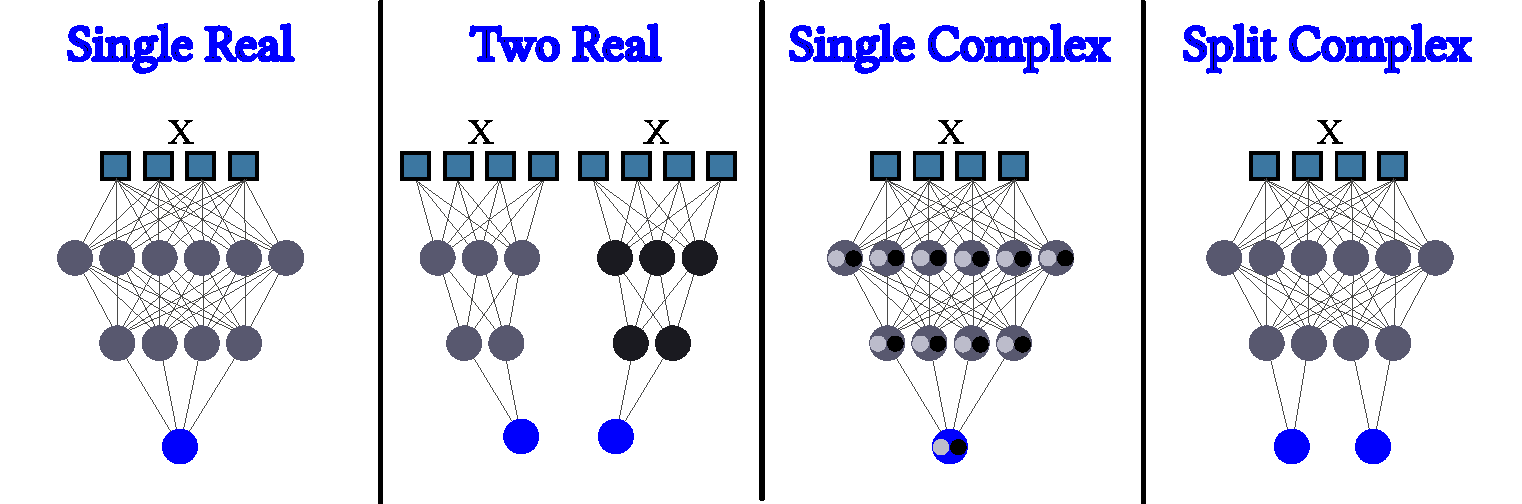
\includegraphics[width=1\textwidth]{./experiments/ground-state-search/ansatz/ansatz.pdf}}
    \caption{
        Schematic visualization of how the four different possibilities for the ansatz are implemented.
        \emph{Single Real} gives a pure real wavefunction output. The architecture is a single network with only real parameters.
        \emph{Two Real} gives a complex wavefunction output (two real numbers, one for the phase and one for the amplitude). The architecture consists of two half-size networks with only real parameters. They do not interact.
        \emph{Single Complex} gives a complex wavefunction output (directly one complex type number). The architecture is a single network with every parameter being a complex number.
        \emph{Split Complex} gives a complex wavefunction output (two real numbers, one for the phase and one for the amplitude). The architecture is a single network with only real parameters, but at the last stage it is split to give two outputs instead of one. The difference to the two real ansatz is that the two \glqq halves\grqq{} of the network can interact.
    }
    \label{fig:ansatz-comparisons}
    
    \makebox[\textwidth][c]{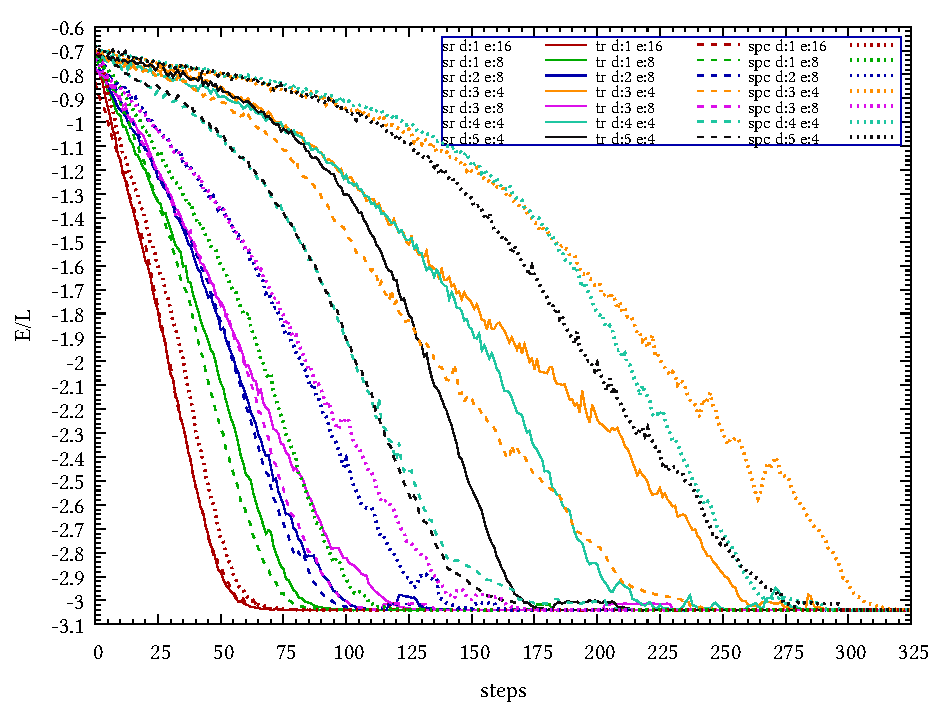
\includegraphics[width=1.1\textwidth]{./experiments/ground-state-search/ansatz/hyperparameter-matrix/hyperparameter-matrix.pdf}}
    \caption{Comparison of hyperparameter combinations. 
            The ansatz is encoded in the dash type, the color specifies the metaformer hyperparameters.
            \emph{sr d:1 e:8} meaning \emph{single real}, \emph{depth 1} and \emph{embed dimension 8}.
            All datasets have been calculated for a randomly encoded \emph{trigonal\_square} lattice with 64 lattice sites.
            Every model is of the type \emph{GPF-NNN} with a mlp-ratio of 4. The Ising parameters are $J=-1$ and $h=-0.7$.
    }
    \label{fig:hyperparameter-matrix}
\end{figure}
        \FloatBarrier
        \subsection{Choice of Hyperparameters}
        \label{sec:experiments-hyperparameters}
        % TODO
        \FloatBarrier
        \subsection{Differences across the Phase Diagram}
        \label{sec:experiments-phasecriticalpoint}
        % TODO
        \FloatBarrier

\chapter{Conclusion}
\label{sec:conclusion}
This thesis serves as an introduction for pure computer scientists to a comparably approachable problem in computational quantum many body physics - \emph{ground state search} with the \emph{transverse field Ising model}.
An outlook into more advanced computational methods like $VMC$ and $DMC$ was given.
This had the intent of motivating aspiring computer scientists with experiences in neural network architectures to take interest in physically motivated calculation problems as opposed to the established task like \emph{natural language processing} or \emph{image classification}.

The general concept of the specialized neural networks of the \emph{metaformer architecture} were explained.
Furthermore these networks were extended to be able to efficiently work on problems that can only be encoded in a \emph{graph} representation and not in the established square tensor format.

The \emph{inductive biases} of different neural network building blocks were presented as a motivation for why the current machine learning calculations operate the way they do.

Solving the \emph{image classification} problem with small networks proved that the envisioned \emph{graph masked attention} was in fact working as expected and possesses the capability to outperform the full transformer by a whole complexity class if implemented properly.
At the same time, the equivalent operations to \emph{convolutions} and \emph{pooling} were introduced and tested for graph representations.

A \emph{ground state search} implementation was modified to support a range of different \emph{2-dimensional lattices}.
The search was first performed with an established \emph{CNN} architecture and validated with the \emph{exact diagonalization} for a problem with a small number of lattice sites.

Finally the graph metaformers were used as the \emph{NQS} for the \emph{VMC} ground state search.
There it could be shown, that the graph architectures can easily be used as a sufficient parameterization for solving the computational search.
And while the graph metaformers were slower in solving the problem compared to the established CNN, the experiments showed them offering a very high degree of customizability due to their structure, good precision and built in resiliency against changes to the graph encoding.

Concluding experiments demonstrated the metaformer's general performance benefits in representing highly complicated wavefunctions, closer to the \emph{phase transition} of quantum mechanical systems.
And while not all variations of the metaformer will always be applicable to discussed computational tasks, already the thesis' small scale experiments have shown the concept to be successful.

Thus, the field of \emph{graph metaformers} and their application in \emph{quantum mechanical computational problems} offers many possibilities for further research, as the vast number of applications sadly surpasses the scope of only one bachelor thesis.

\FloatBarrier

% ! Addendum
\newpage
\nocite{*}
\printbibliography[title={Bibliography}]
\chapter{Appendix}
\label{sec:appendix}

%! needs to be first, because of format adapted to chapter title of appendix
\section{Lattice Visualization} \label{appendix:lattice-visualisation}

\begin{minipage}{\linewidth}
    \centering
    \makebox[\textwidth][c]{
        \makebox[1.25\textwidth][c]{
            \makebox[0.40\textwidth][l]{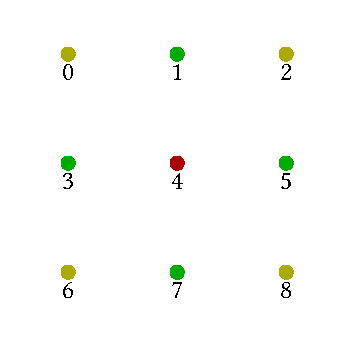
\includegraphics[width=0.33\textwidth]{./../appendix/lattice_visualization/square,size=2,np.pdf}}
            \makebox[0.40\textwidth][l]{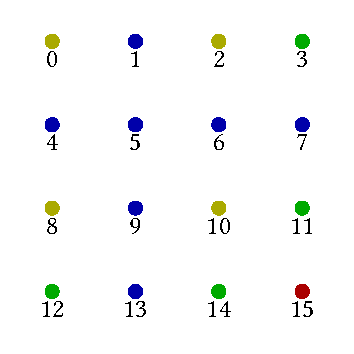
\includegraphics[width=0.33\textwidth]{./../appendix/lattice_visualization/square,size=3,p.pdf}}
            \makebox[0.40\textwidth][l]{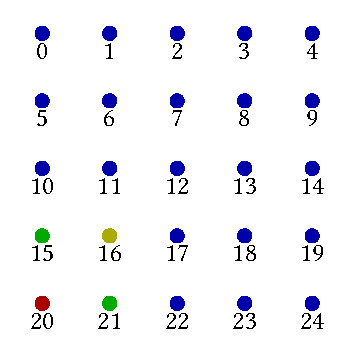
\includegraphics[width=0.33\textwidth]{./../appendix/lattice_visualization/square,size=4,np.pdf}}
        }
    }

    \captionof{figure}{A visualization of the \textbf{2D-square} lattice structure, measured in this thesis. 
        The lattices from left to right can be described by the parameters\\
        1: \emph{size=2, non-periodic}\,\,\,\, 2: \emph{size=3, periodic}\,\,\,\, 3: \emph{size=4, non-periodic}
    }
    \label{fig:appendix-square-lattices}
\end{minipage}

\vspace{0.5cm}

\begin{minipage}{\linewidth}
    \centering
    \makebox[\textwidth][c]{
        \makebox[1.25\textwidth][c]{
            \makebox[0.40\textwidth][l]{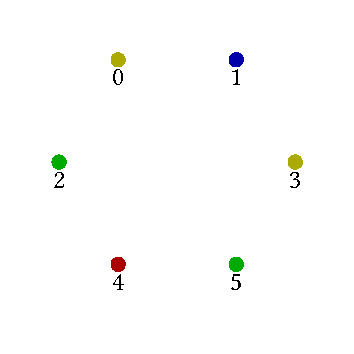
\includegraphics[width=0.33\textwidth]{./../appendix/lattice_visualization/hexagonal,size=1,np.pdf}}
            \makebox[0.40\textwidth][l]{\includegraphics[width=0.33\textwidth]{./../appendix/lattice_visualization/hexagonal,size=2,np.pdf}}
            \makebox[0.40\textwidth][l]{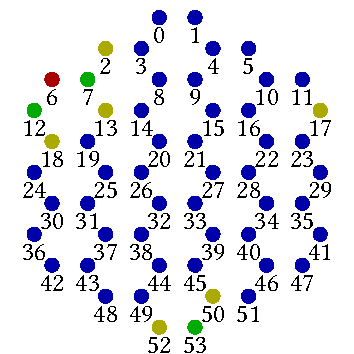
\includegraphics[width=0.33\textwidth]{./../appendix/lattice_visualization/hexagonal,size=3,p.pdf}}
        }
    }

    \vspace{0.3cm}
    \captionof{figure}{A visualization of the \textbf{2D-hexagonal} lattice structure, measured in this thesis. 
        The lattices from left to right can be described by the parameters \\
        1: \emph{size=1, non-periodic}\,\,\,\, 2: \emph{size=2, non-periodic}\,\,\,\, 3: \emph{size=3, periodic}
    }
    \label{fig:appendix-hexagonal-lattices}
\end{minipage}

\vspace{0.4cm}

\begin{minipage}{\linewidth}
    \centering
    \makebox[\textwidth][c]{
        \makebox[1.25\textwidth][c]{
            \makebox[0.40\textwidth][l]{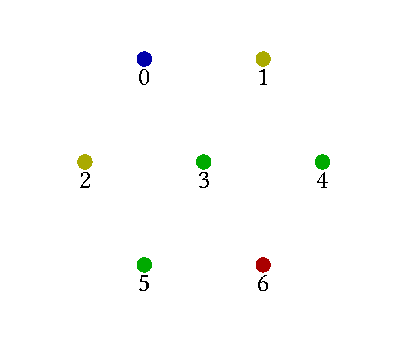
\includegraphics[width=0.33\textwidth]{./../appendix/lattice_visualization/trigonal_hexagonal,size=1,np.pdf}}
            \makebox[0.40\textwidth][l]{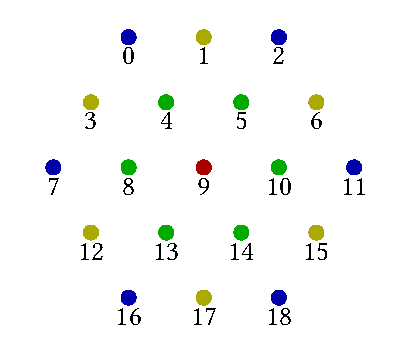
\includegraphics[width=0.33\textwidth]{./../appendix/lattice_visualization/trigonal_hexagonal,size=2,np.pdf}}
            \makebox[0.40\textwidth][l]{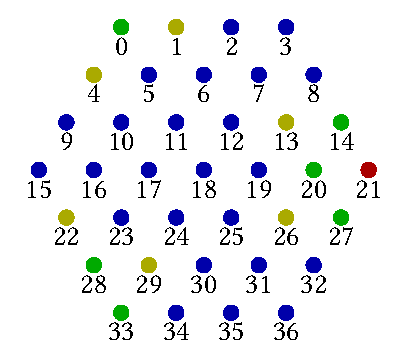
\includegraphics[width=0.33\textwidth]{./../appendix/lattice_visualization/trigonal_hexagonal,size=3,p.pdf}}
        }
    }
    
    \vspace{0.5cm}
    \captionof{figure}{A visualization of the \textbf{2D-trigonal\_hexagonal} lattice structure, measured in this thesis. 
        The lattices from left to right can be described by the parameters \\
        1: \emph{size=1, non-periodic}\,\,\,\, 2: \emph{size=2, non-periodic}\,\,\,\, 3: \emph{size=3, periodic}
    }
    \label{fig:appendix-trigonal_hexagonal-lattices}
\end{minipage}

% HERE SHOULD THE PAGE-BREAK BE. i love latex, but stuff like this infuriates me to get correct
\newpage
\makebox{\vspace{5cm}}\\

\begin{minipage}{\linewidth}
    \centering
    \makebox[\textwidth][c]{
        \makebox[1.25\textwidth][c]{
            \makebox[0.40\textwidth][l]{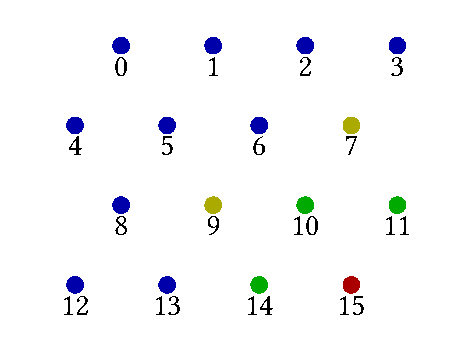
\includegraphics[width=0.33\textwidth]{./../appendix/lattice_visualization/trigonal_square,size=2,np.pdf}}
            \makebox[0.40\textwidth][l]{\includegraphics[width=0.33\textwidth]{./../appendix/lattice_visualization/trigonal_square,size=3,np.pdf}}
            \makebox[0.40\textwidth][l]{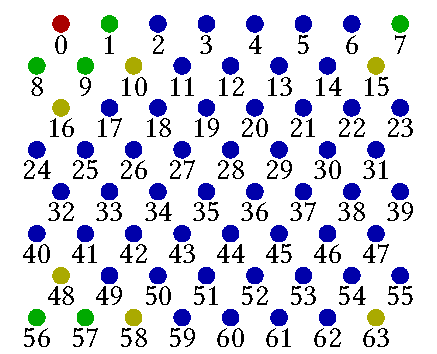
\includegraphics[width=0.33\textwidth]{./../appendix/lattice_visualization/trigonal_square,size=4,p.pdf}}
        }
    }

    \vspace{0.4cm}
    \captionof{figure}{A visualization of the \textbf{2D-trigonal\_square} lattice structure, measured in this thesis. 
        The lattices from left to right can be described by the parameters \\
        1: \emph{size=2, non-periodic}\,\,\,\, 2: \emph{size=3, non-periodic}\,\,\,\, 3: \emph{size=4, periodic}
    }
    \label{fig:appendix-trigonal_square-lattices}
\end{minipage}

\vspace{1.2cm}

\begin{minipage}{\linewidth}
    \centering
    \makebox[\textwidth][c]{
        \makebox[1.25\textwidth][c]{
            \makebox[0.40\textwidth][c]{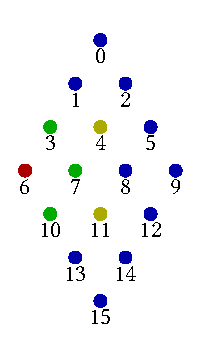
\includegraphics[width=0.20\textwidth]{./../appendix/lattice_visualization/trigonal_diamond,size=3,np.pdf}}
            \makebox[0.40\textwidth][c]{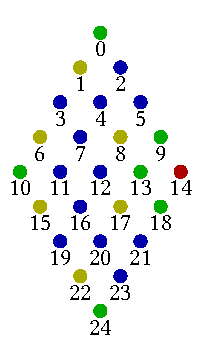
\includegraphics[width=0.20\textwidth]{./../appendix/lattice_visualization/trigonal_diamond,size=4,p.pdf}}
            \makebox[0.40\textwidth][c]{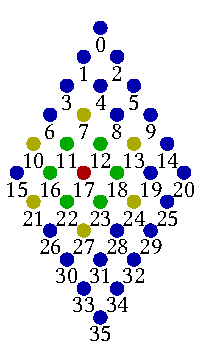
\includegraphics[width=0.20\textwidth]{./../appendix/lattice_visualization/trigonal_diamond,size=5,np.pdf}}
        }
    }

    \vspace{0.4cm}
    \captionof{figure}{A visualization of the \textbf{2D-trigonal\_diamond} lattice structure, measured in this thesis. 
        The lattices from left to right can be described by the parameters \\
        1: \emph{size=3, non-periodic}\,\,\,\, 2: \emph{size=4, periodic}\,\,\,\, 3: \emph{size=5, non-periodic}
    }
    \label{fig:appendix-trigonal_diamond-lattices}
\end{minipage}

\vspace{1.2cm}

\begin{minipage}{\linewidth}
    \centering
    \makebox[\textwidth][c]{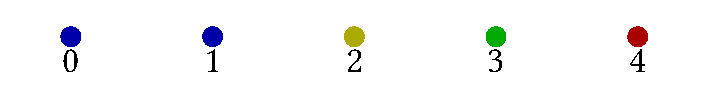
\includegraphics[width=0.80\textwidth]{./../appendix/lattice_visualization/linear,size=5,np.pdf}}
    \vspace*{0.2cm}
    \makebox[\textwidth][c]{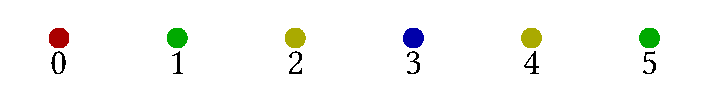
\includegraphics[width=0.80\textwidth]{./../appendix/lattice_visualization/linear,size=6,p.pdf}}
    \vspace*{0.2cm}
    \makebox[\textwidth][c]{
\includegraphics[width=0.80\textwidth]{./../appendix/lattice_visualization/linear,size=8,np.pdf}}

    \vspace{0.2cm}
    \captionof{figure}{A visualization of the \textbf{1D-linear} lattice structure, measured in this thesis. 
        The lattices from top to bottom can be described by the parameters \\
        1: \emph{size=5, non-periodic}\,\,\,\, 2: \emph{size=6, periodic}\,\,\,\, 3: \emph{size=8, non-periodic}
    }
    \label{fig:appendix-linear-lattices}
\end{minipage}

\newpage

% pdf as a additional information, can be nicely ref-ed ("\fullpage{anhang:test}") because of fake section that doesn't get shown in the table of contents
% \includepdf[pagecommand={\section*{} \label{appendix:test}}]{appendix/test.pdf}

% minted to properly import and style code. ! Needs python libraries
\newpage
\section{Dot Product Self Attention (jax)} \label{appendix:attention}
    \cite{selfPhysics}, \filepath{/models/metaformer.py}
    \inputminted[firstline=149, lastline=169]{python}{./../physics-code/models/metaformer.py}

\section{Graph Conformer Module (jax)} \label{appendix:graph-conformer}
    \cite{selfPhysics}, \filepath{/models/metaformer.py}
    \inputminted[firstline=242, lastline=284]{python}{./../physics-code/models/metaformer.py}

\newpage
\section{Graph Poolformer Module (jax)} \label{appendix:graph-poolformer}
    \cite{selfPhysics}, \filepath{/models/metaformer.py}
    \inputminted[firstline=211, lastline=239]{python}{./../physics-code/models/metaformer.py}
    

\end{document}





